This chapter provides a detailed, step-by-step blueprint of the research design and analytical framework used to compare the traditional and machine learning-based calibration methods. The process begins with a thorough description of the dataset, which includes European \ac{atm} swaptions, the underlying \ac{eur} swap curves, and key external market indicators like the \ac{vix} and \ac{move} indices.

From this raw data, a sophisticated set of features is engineered through a multi-stage preprocessing pipeline. This includes bootstrapping zero-coupon curves, handling non-trading days, and using \ac{pca} to distill the yield curve's primary drivers, level, slope, and curvature, into a compact and uncorrelated feature set.

The core of the methodology is the end-to-end machine learning pipeline. This section details the \ac{nn}'s residual architecture, the systematic hyperparameter optimization conducted via the Hyperband algorithm, and the implementation of a custom, asymmetric loss function designed to penalize the underestimation of volatility. Furthermore, it addresses the significant technical challenge of integrating the differentiable TensorFlow framework with the non-differentiable QuantLib pricing engine through the use of custom gradients and parallelized computation.

Crucially, the chapter concludes by defining the rigorous experimental protocol established for the final comparison. It details the unique "Intra-Day Hold-Out Set" framework, which was specifically designed to ensure a scientifically valid and fair out-of-sample evaluation for both the predictive \ac{nn} and the in-sample \ac{lm} optimizer, thereby addressing a fundamental methodological challenge in comparing these two distinct approaches.

\subsection{Dataset}
\subsubsection{Time Period}
The market data used for the calibration of the one-factor \ac{hw} model covers a continuous time span of 92 calendar days, from June 1, 2025, to August 31, 2025. Observations are available for each calendar day within this period; weekends and public holidays are not excluded. All market snapshots were collected at a daily frequency, ensuring a consistent temporal resolution across the entire observation window.

\subsubsection{Swaptions}
The calibration is based on a comprehensive panel of European \ac{atm} payer and receiver swaptions quoted in the \ac{eur} market. Each daily market snapshot consists of a complete normal volatility surface containing 228 distinct volatility points, derived from combinations of option maturities and underlying swap tenors.

The set of option maturities includes:
1 month, 3 months, 9 months, 1 year, 2 years, 3 years, 4 years, 5 years, 6 years, 7 years, 8 years, 9 years, 10 years, 12 years, 15 years, 20 years, 25 years, and 30 years.

The corresponding underlying swap tenors are:
1 year, 2 years, 3 years, 4 years, 5 years, 7 years, 10 years, 12 years, 15 years, 20 years, 25 years, and 30 years.

The floating leg of each underlying swap resets on a semiannual (6-month) basis. Volatilities are quoted in normal (Bachelier) terms, expressed in \ac{bps} of the underlying swap rate, and represent the mid-market levels (average of bid and ask quotes). Only \ac{atm} swaptions are considered in the calibration.

All swaption data were obtained from Bloomberg using the \texttt{VCUB} function with \texttt{BVOL} as the source. Due to the university's Bloomberg license restrictions, direct data downloads were not permitted; therefore, the data were captured via screenshots and subsequently converted into Excel format for processing. Bloomberg employs the \ac{eur} OIS (ESTR) discounting curve, identified as \texttt{(514) \ac{eur} OIS (ESTR)}, and the \ac{eur} swap curve \texttt{(45) Euro} for the construction of the volatility cube. This ensures internal consistency between the volatility and yield curve data used in the \ac{hw} model calibration.

\subsubsection{Swap Curves}
The initial yield curves employed for the \ac{hw} model calibration are derived from the \ac{eur} (vs. 6M \ac{euribor}) Swap / Projection Curve, identified in Bloomberg as \texttt{45}. This curve represents a forward (projection) curve used to generate 6-month \ac{euribor} forward rates for pricing and valuation. The discounting is performed using the \ac{eur} OIS (ESTR) curve (\texttt{Bloomberg ID 514}), consistent with the multi-curve framework applied in current market practice.

The market instruments used in the bootstrapping of the projection curve include:
\begin{itemize}
	\item Cash deposits: Overnight to 12-month maturities, anchoring the short end of the curve.
	\item \ac{fra}: Typically spanning 1×7 to 9×15 months, bridging the short and medium-term maturities.
	\item Interest-rate swaps: Par fixed-vs-6M \ac{euribor} swaps from 1 year up to 30 years, forming the long end of the term structure.
\end{itemize}

Day-count conventions follow market standards: ACT/360 for short and medium maturities and 30U/360 for the long end. All market quotes correspond to mid (bid/ask midpoint) levels. The market data source is the Bloomberg Generic (BGN) composite, which aggregates dealer contributions to provide representative market levels.

The curve is bootstrapped sequentially from cash deposits through \ac{fra}s to interest-rate swaps, producing a continuous zero rate and forward rate term structure. The interpolation is typically performed in a log-linear fashion on either discount factors or zero rates. Within the Bloomberg volatility cube environment (\texttt{VCUB}), this curve appears as \texttt{Swap Curve (45) Euro} and provides consistent forward rate inputs for the calibration of EUR 6M swaption volatilities.

\subsubsection{MOVE Index}
The \ac{move} index represents the treasury market's implied volatility and serves as a primary external indicator of interest rate uncertainty. Daily open values of the \ac{move} index were collected from Yahoo Finance to capture the most up-to-date measure of market-implied interest rate volatility at the start of each trading day. By using the open rather than closing values, the \ac{nn} is able to predict \ac{hw} model parameters early in the day, leveraging the most recent available information without waiting for end-of-day data. The \ac{move} index is particularly relevant as it captures expected fluctuations in interest rates, which directly influence the calibration of the \ac{hw} model.

\subsubsection{Volatility Index}
The \ac{vix} provides a widely recognized measure of equity market implied volatility and serves as a general gauge of market fear and risk appetite. Daily open values of the \ac{vix} were downloaded from Yahoo Finance to reflect the initial market sentiment for each trading day. High \ac{vix} levels, indicative of a "risk-off" environment, can have spillover effects on bond and swap markets, thereby indirectly affecting European interest rates. Including \ac{vix} open values in the dataset allows the \ac{nn} to incorporate contemporaneous equity market volatility into the prediction of \ac{hw} parameters, potentially improving model responsiveness to market stress conditions.

\subsubsection{EUR/USD Exchange Rate}
The EUR/USD exchange rate reflects the relative economic and monetary conditions between the Eurozone and the United States. Daily open prices were obtained from Yahoo Finance to capture the most current cross-currency market information at the start of each trading day. Large movements in the EUR/USD rate may indicate capital flows or diverging monetary policy actions between the European Central Bank and the Federal Reserve, which have direct implications for European interest rates. By including the open EUR/USD rate in the feature set, the \ac{nn} can incorporate up-to-date foreign exchange market dynamics when predicting \ac{hw} model parameters.

\subsection{Descriptive Analysis of Market and Model Inputs}
This section provides a detailed examination of the key figures illustrating the underlying financial data and model inputs used in this study. Each figure is analyzed with respect to its economic interpretation and its implications for the modeling framework.

\begin{figure}[H]
	\centering
	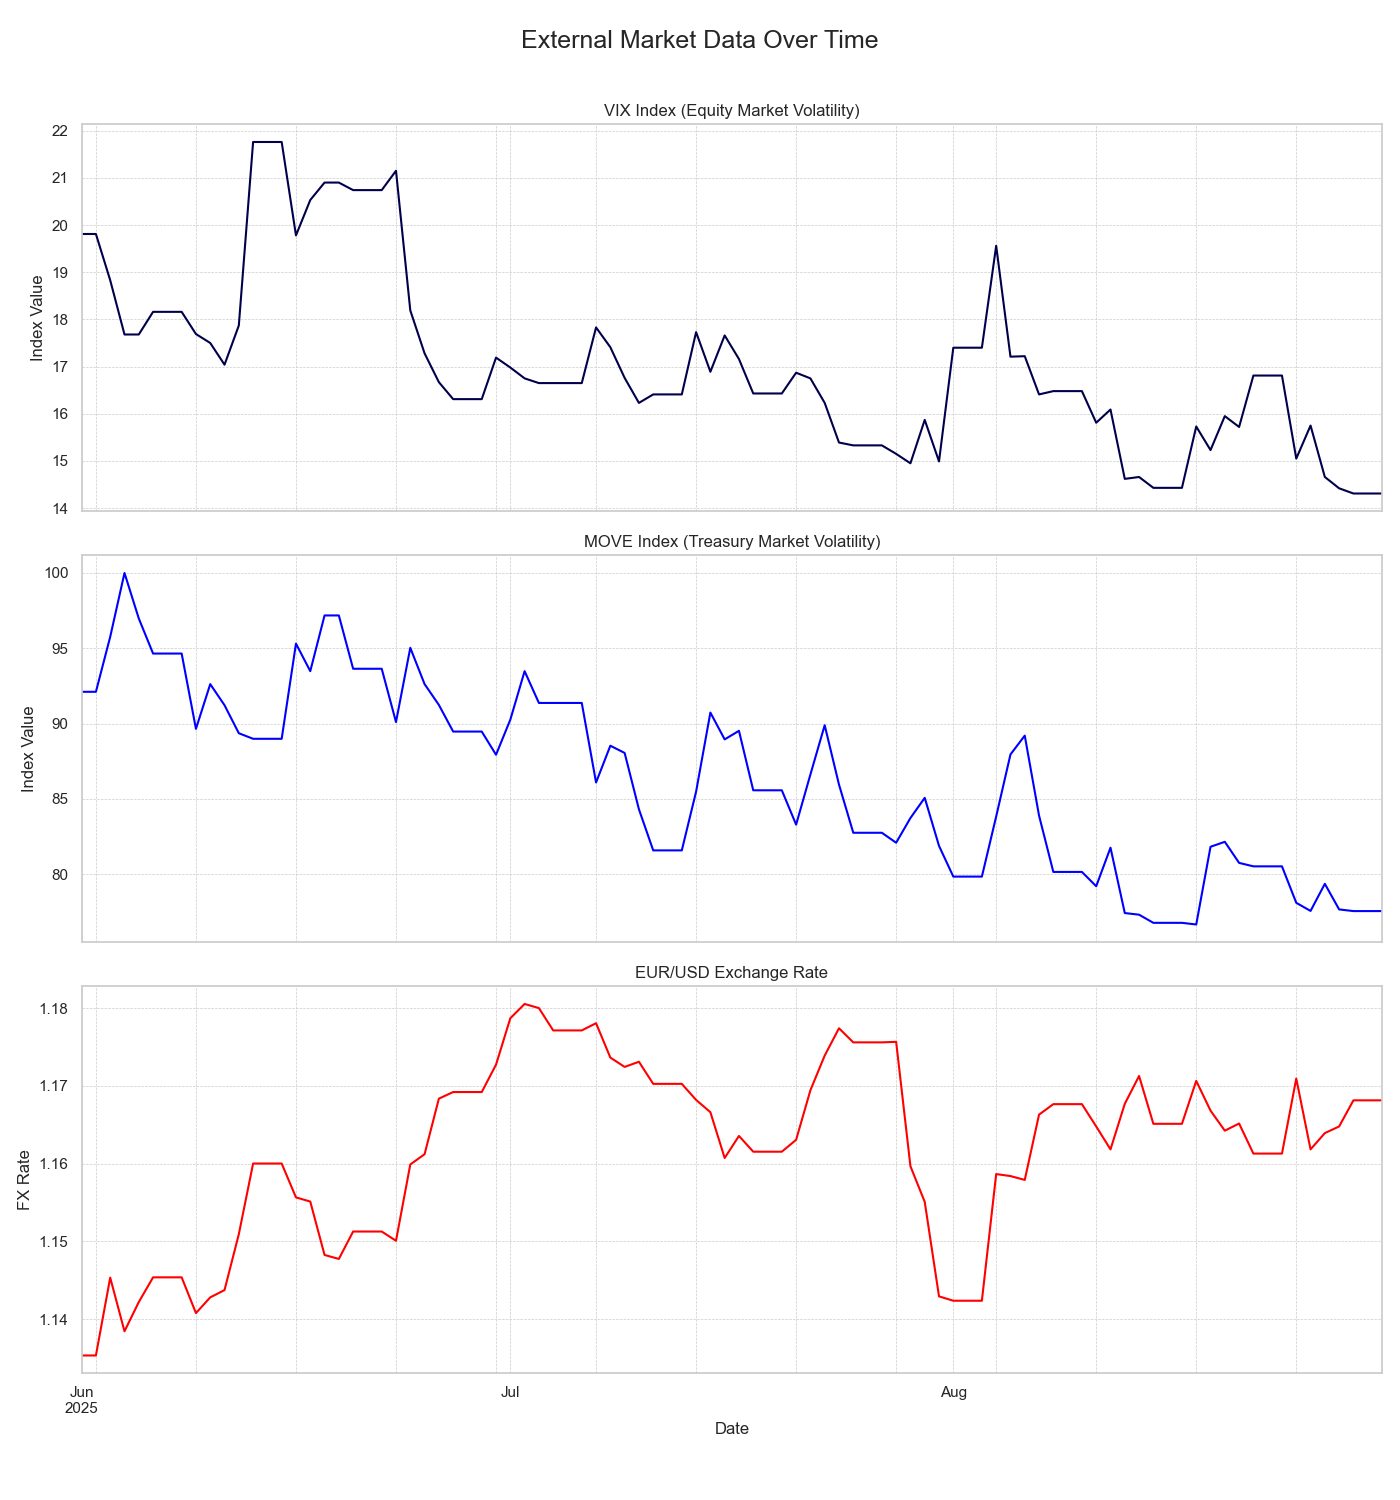
\includegraphics[width=1\textwidth]{images/descriptive_data_analysis/external_data_time_series.png}
	\caption{Time Series of Market-Wide Indicators (VIX, MOVE, and EUR/USD)}
	\label{fig:external_data_time_series}
\end{figure}

Figure~\ref{fig:external_data_time_series} depicts the evolution of key market indicators between June and late August 2025. The overall market environment during this period is characterized by a notable decrease in volatility across major asset classes. The \textit{VIX}, representing equity market volatility, begins near a relatively elevated level of 20 before declining sharply in late June and stabilizing within a range of 14-17. This pattern suggests a reduction in perceived equity market risk. Similarly, the \textit{MOVE Index}, a measure of treasury market volatility, exhibits an even more pronounced decline, from approximately 100 to below 80, indicating a substantial calming of interest rate expectations. Concurrently, the \textit{EUR/USD} exchange rate shows a strengthening of the Euro against the \ac{usd}, peaking near 1.18 in mid-July before a modest correction. These co-evolving patterns reflect a broad reduction in cross-asset risk and uncertainty.

% --- TABLE 1 INSERTED HERE ---
\begin{table}[H]
	\centering
	\begin{threeparttable}
		\caption{Summary Statistics of External Market Factors}
		\label{tab:external_summary}
		\begin{tabular}{lccccc}
			\toprule
			\textbf{Factor} & \textbf{Mean} & \textbf{Median} & \textbf{Std. Dev.} & \textbf{Skewness} & \textbf{Kurtosis} \\
			\midrule
			\ac{vix}        & 17.05         & 16.71           & 1.89               & 0.89              & 0.34              \\
			\ac{move} Index & 86.29         & 86.02           & 6.12               & 0.10              & -1.10             \\
			EUR/USD Rate    & 1.162         & 1.164           & 0.011              & -0.57             & -0.54             \\
			\bottomrule
		\end{tabular}
		\begin{tablenotes}
			\footnotesize
			\item  A summary of the key external market factors over the analysis period. The positive skew in the \ac{vix} and the non-zero kurtosis across all factors suggest deviations from a normal distribution.
		\end{tablenotes}
	\end{threeparttable}
\end{table}


Table~\ref{tab:external_summary} provides a quantitative summary of the external market factors depicted in figure~\ref{fig:external_data_time_series}. The statistics confirm the visual analysis, detailing the central tendency and dispersion of each series. Notably, the \ac{vix} exhibits significant positive skewness (0.89), indicating that upward spikes in volatility are more pronounced than downward movements. Conversely, the EUR/USD rate shows a negative skew (-0.57). The kurtosis values, which deviate from the zero value of a mesokurtic distribution, provide further numerical evidence that these financial time series are not normally distributed, a crucial consideration for the modeling approach.

\begin{figure}[H]
	\centering
	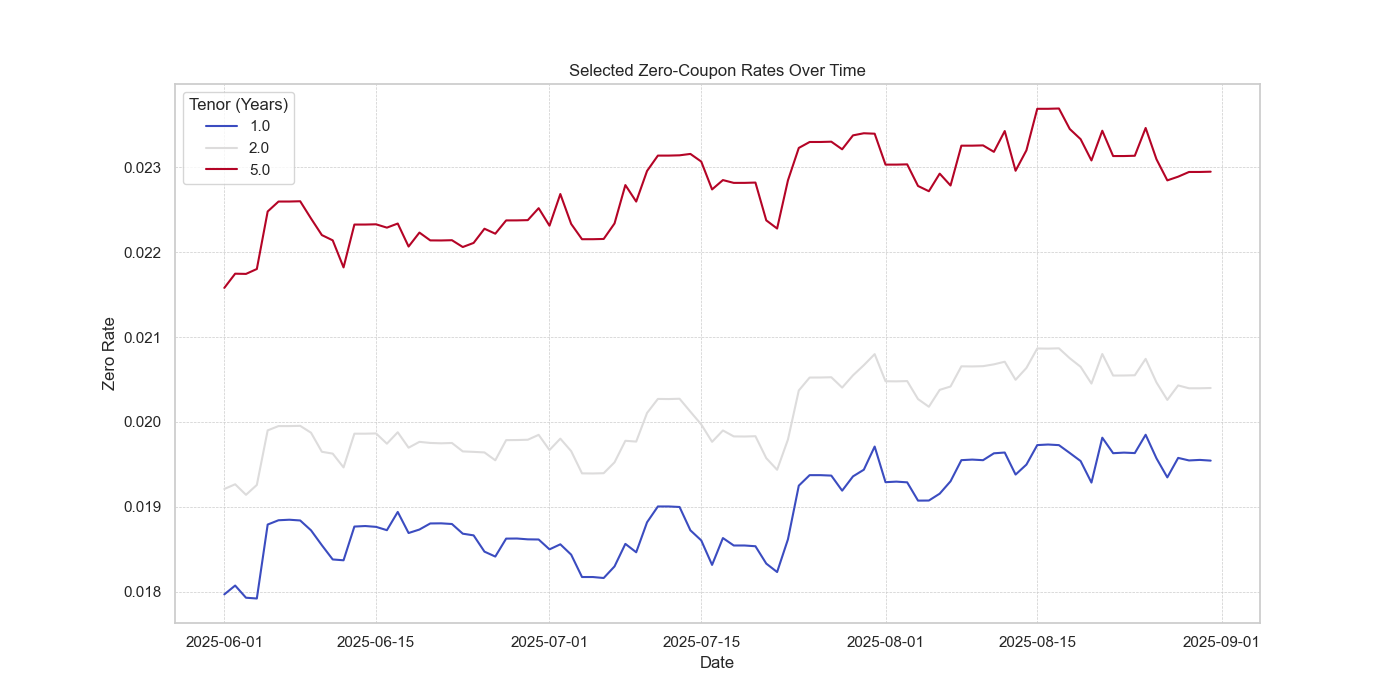
\includegraphics[width=1\textwidth]{images/descriptive_data_analysis/yield_curve_selected_tenors.png}
	\caption{Yield Curve Dynamics for Selected Tenors (1Y, 2Y, 5Y)}
	\label{fig:yield_curve_selected_tenors}
\end{figure}

Figure~\ref{fig:yield_curve_selected_tenors} illustrates the time series of yields across selected maturities. The yield curve retains its normal, upward-sloping shape throughout the observation window. A gradual upward shift is visible across all tenors, indicating a moderate tightening of monetary conditions. The largely parallel movement across maturities implies that changes are predominantly driven by a “level” factor. Minor deviations in spreads, however, suggest that “slope” and “curvature” components contribute modestly to the curve's dynamics.

\begin{figure}[H]
	\centering
	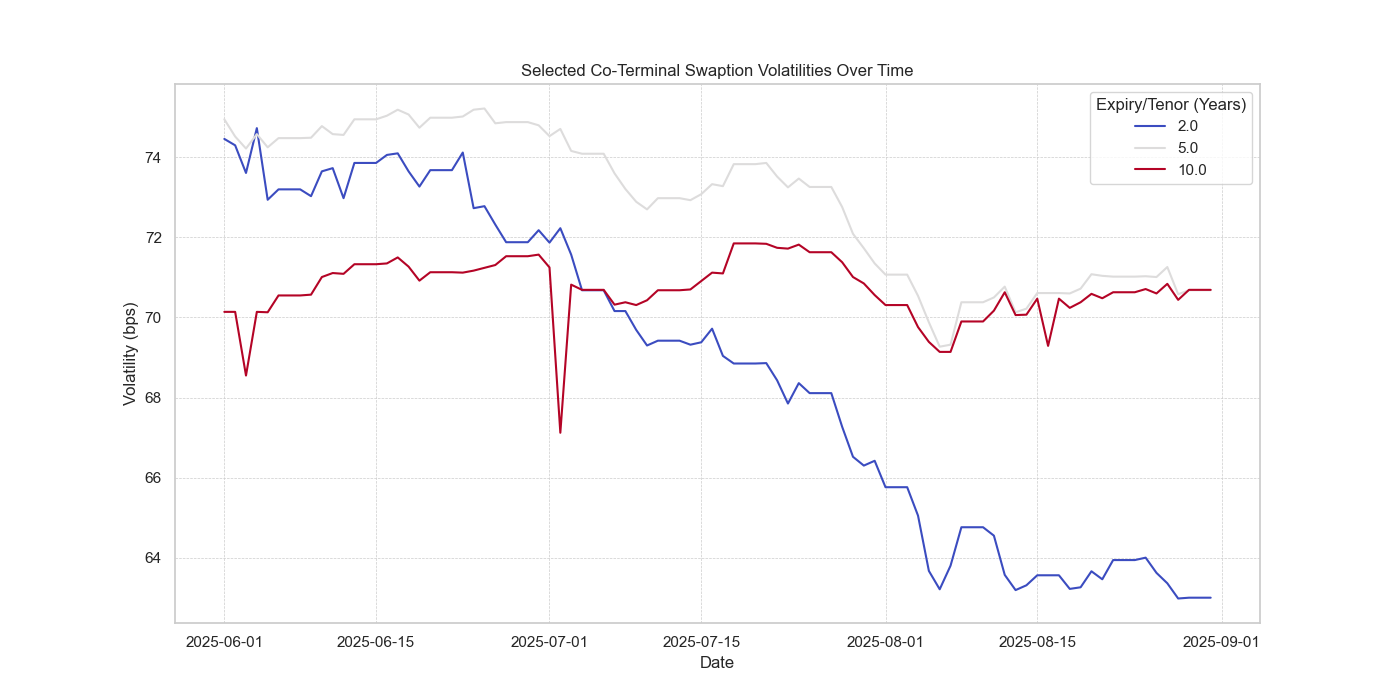
\includegraphics[width=1\textwidth]{images/descriptive_data_analysis/vol_surface_coterminal_series.png}
	\caption{Time Series of Coterminal Swaption Volatilities}
	\label{fig:vol_surface_coterminal_series}
\end{figure}

Figure~\ref{fig:vol_surface_coterminal_series} presents the evolution of the coterminal swaption volatility term structure. The curve is generally downward sloping, with shorter maturities exhibiting higher volatility levels than longer maturities. The short-term (2-year) volatility declines sharply from over 74~\ac{bps} to approximately 63~\ac{bps}, whereas the long-term (10-year) volatility remains comparatively stable. This differential behavior leads to a pronounced flattening of the volatility term structure-a key empirical feature that any robust model should accurately capture.

\begin{figure}[H]
	\centering
	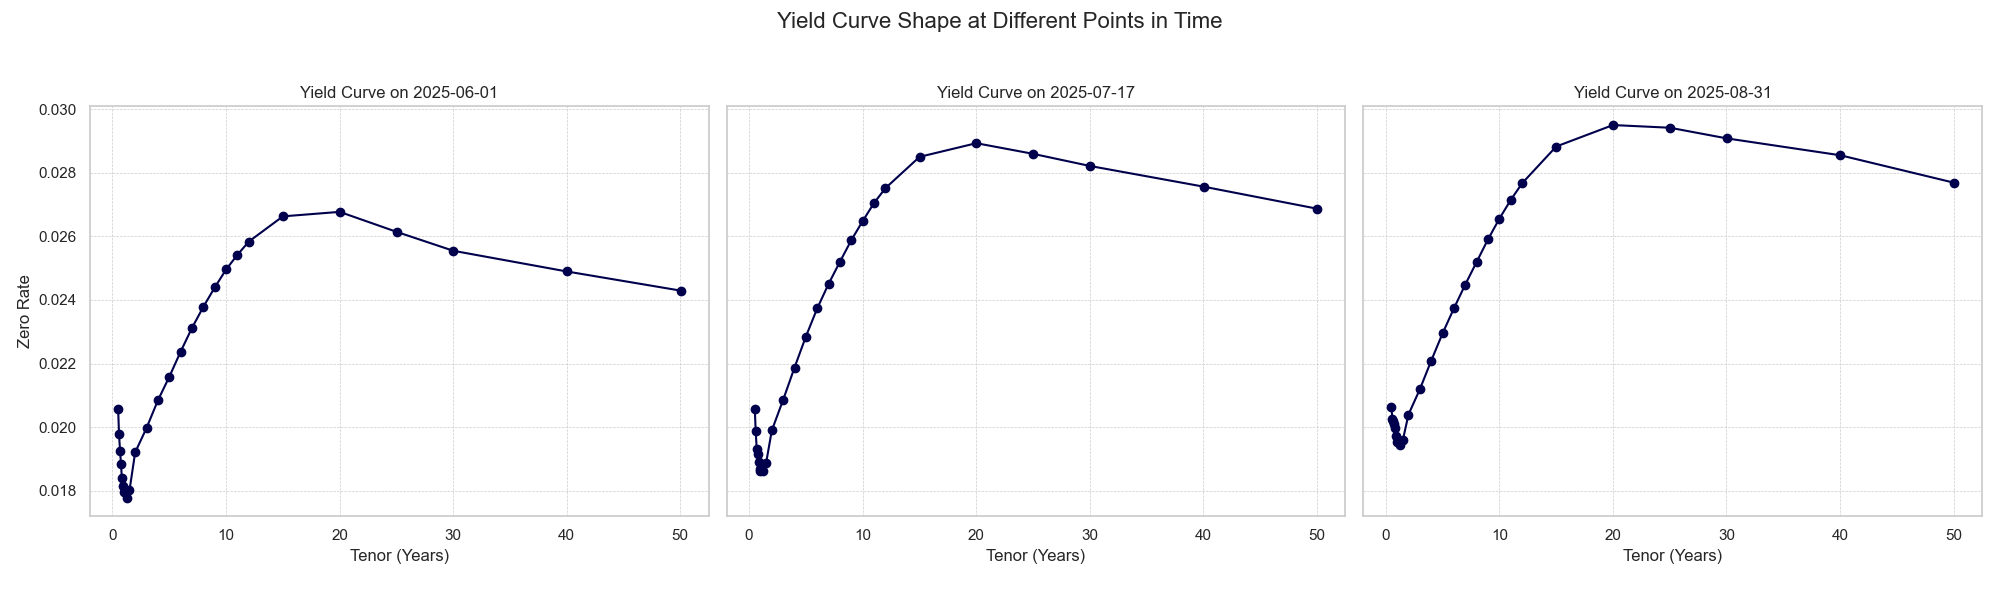
\includegraphics[width=1\textwidth]{images/descriptive_data_analysis/yield_curve_2d_snapshots.png}
	\caption{Yield Curve Snapshots over Time}
	\label{fig:yield_curve_2d_snapshots}
\end{figure}

Figure~\ref{fig:yield_curve_2d_snapshots} visualizes static yield curve snapshots at different points in time. The yield curve consistently displays a concave, upward-sloping shape, typical for stable economic environments. The entire curve shifts upward from June to August, reinforcing the observed trend of rising interest rates. Moreover, the curvature appears to increase slightly over time, suggesting subtle changes in the underlying term structure dynamics.

\begin{table}[H]
	\centering
	\begin{threeparttable}
		\caption{Descriptive Statistics for Key Yield Curve Tenors}
		\label{tab:yield_curve_summary}
		\begin{tabular}{lcccc}
			\toprule
			\textbf{Tenor} & \textbf{Mean Rate (\%)} & \textbf{Std. Dev. (\%)} & \textbf{Skewness} & \textbf{Kurtosis} \\
			\midrule
			1-Year         & 1.90                    & 0.05                    & -0.02             & -1.10             \\
			5-Year         & 2.27                    & 0.05                    & -0.18             & -0.88             \\
			10-Year        & 2.62                    & 0.06                    & -0.25             & -1.04             \\
			30-Year        & 2.76                    & 0.12                    & -0.29             & -1.22             \\
			\bottomrule
		\end{tabular}
		\begin{tablenotes}
			\footnotesize
			\item  Descriptive statistics for selected benchmark tenors of the zero-coupon yield curve. Mean Rate and Standard Deviation are expressed in percentage points.
		\end{tablenotes}
	\end{threeparttable}
\end{table}

Table~\ref{tab:yield_curve_summary} quantifies the characteristics of the yield curve by presenting descriptive statistics for key benchmark tenors. The increasing mean rate with tenor numerically confirms the upward-sloping nature of the term structure. A particularly important finding is the behavior of the standard deviation, which increases from 0.05\% for the 1-year rate to 0.12\% for the 30-year rate. This demonstrates that the long end of the yield curve is substantially more volatile in absolute terms, a stylized fact that is further explored in figure~\ref{fig:yield_curve_std_by_tenor}.

\begin{figure}[H]
	\centering
	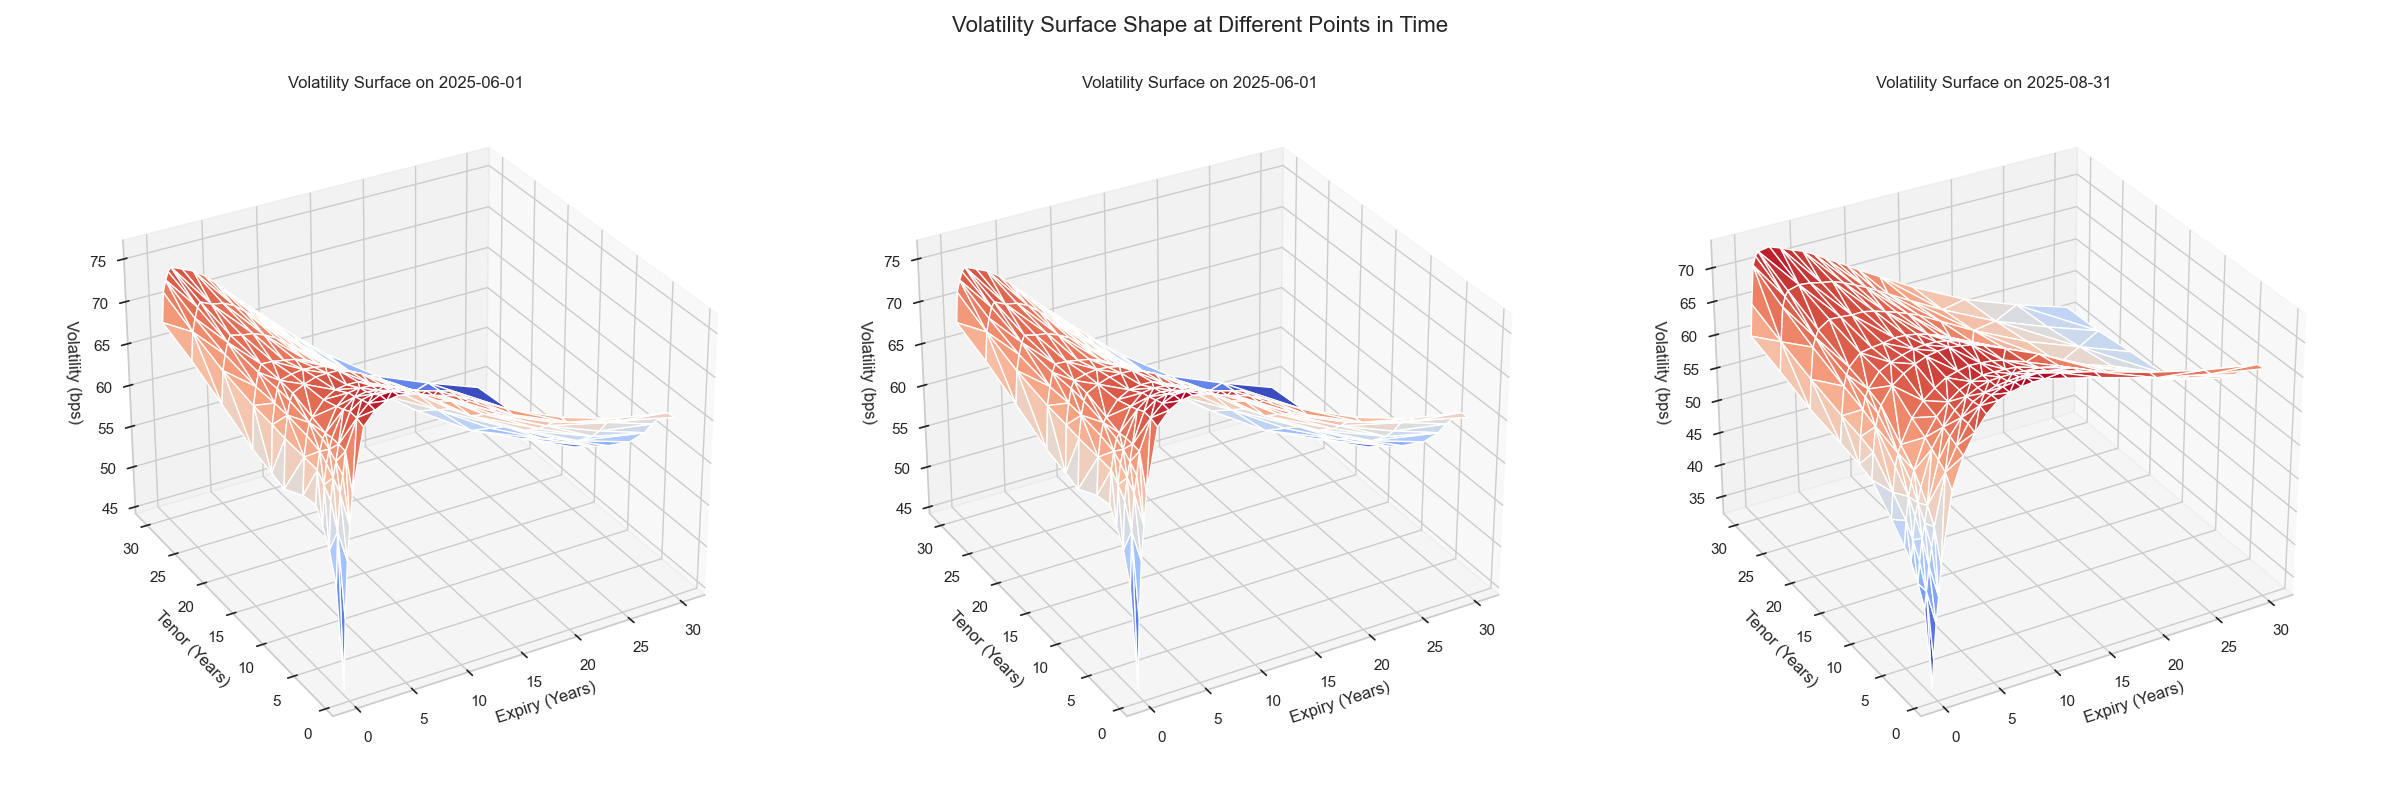
\includegraphics[width=1\textwidth]{images/descriptive_data_analysis/vol_surface_3d_snapshots.png}
	\caption{3D Representation of the Swaption Volatility Surface}
	\label{fig:vol_surface_3d_snapshots}
\end{figure}

Figure~\ref{fig:vol_surface_3d_snapshots} provides a three-dimensional representation of the swaption volatility surface. The surface exhibits pronounced structure, with the highest volatilities concentrated in short-expiry, short-tenor instruments. Volatility decreases along both the expiry and tenor dimensions, forming a characteristic “hump” at the short end. This structural complexity underscores the necessity of employing non-linear modeling approaches-such as \ac{nn}s-to accurately capture the surface's intricate shape and temporal dynamics.

\begin{figure}[H]
	\centering
	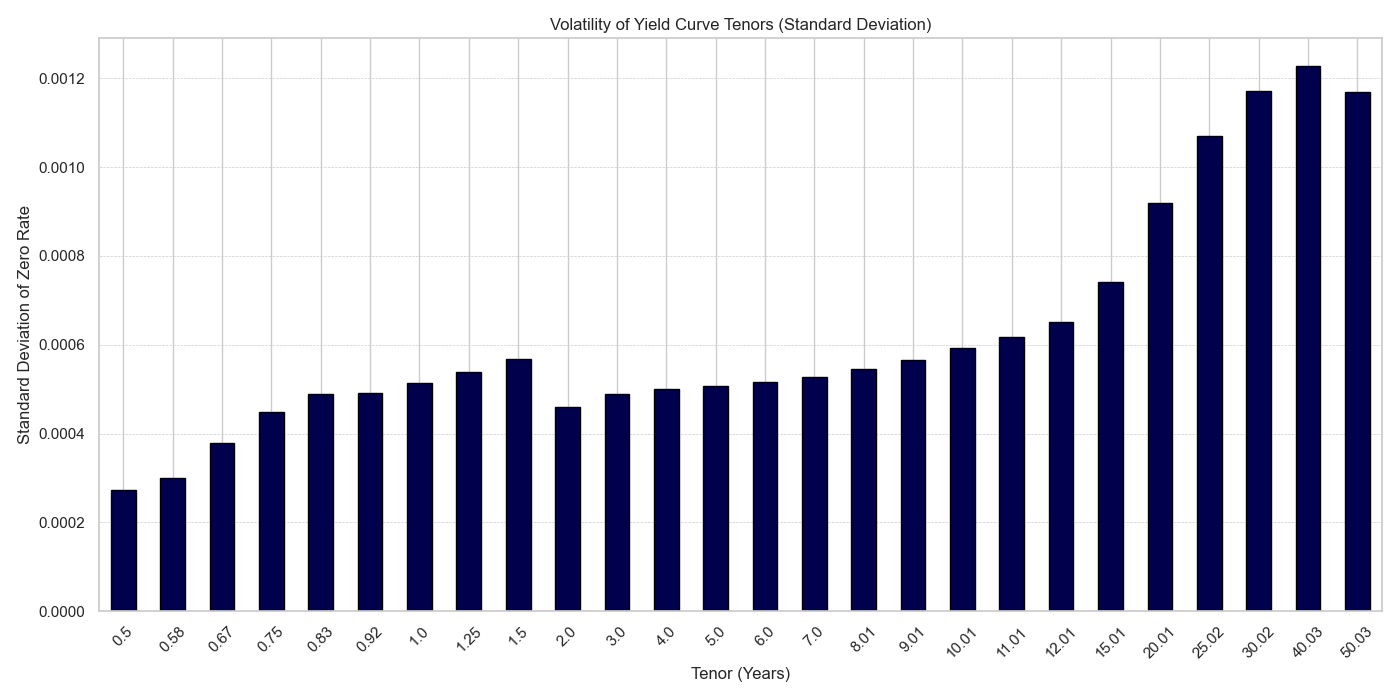
\includegraphics[width=1\textwidth]{images/descriptive_data_analysis/yield_curve_std_by_tenor.png}
	\caption{Standard Deviation of Daily Yield Changes by Tenor}
	\label{fig:yield_curve_std_by_tenor}
\end{figure}

Figure~\ref{fig:yield_curve_std_by_tenor} shows the distribution of yield volatility across maturities. Volatility is lowest at the short end, increases moderately in the 1-2 year range, and rises significantly for longer maturities beyond 10 years. This pattern highlights that long-term yields exhibit the greatest absolute variability, a crucial consideration for risk management and model calibration.

\begin{figure}[H]
	\centering
	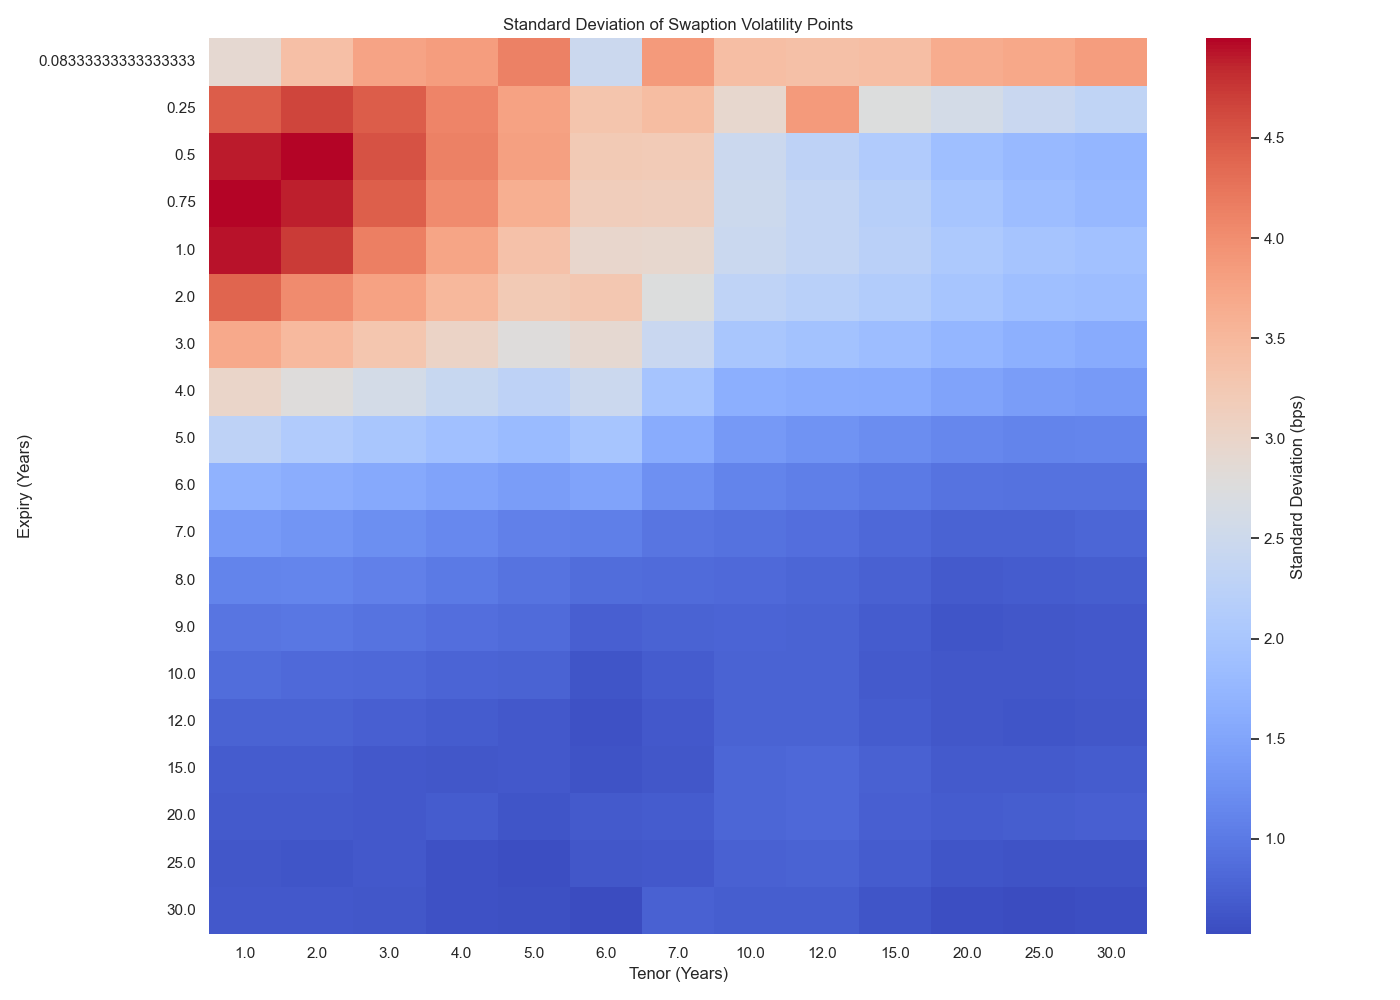
\includegraphics[width=1\textwidth]{images/descriptive_data_analysis/vol_surface_std_heatmap.png}
	\caption{Heatmap of Swaption Volatility Surface Standard Deviations}
	\label{fig:vol_surface_std_heatmap}
\end{figure}

Figure~\ref{fig:vol_surface_std_heatmap} displays the standard deviation of swaption volatilities across expiry and tenor dimensions. The highest volatility, represented by the most intense red shading, is concentrated in the short-expiry, short-tenor region. This indicates that the front end of the surface is particularly unstable, while the long end remains relatively static. A well-performing model must therefore excel at capturing the pronounced temporal variability in this region.

\begin{table}[H]
	\centering
	\begin{threeparttable}
		\caption{Standard Deviation of Swaption Volatilities (in \ac{bps})}
		\label{tab:vol_std_summary}
		\begin{tabular}{lcccc}
			\toprule
			\textbf{Expiry} & \textbf{1-Year Tenor} & \textbf{5-Year Tenor} & \textbf{10-Year Tenor} & \textbf{30-Year Tenor} \\
			\midrule
			1-Year          & 4.93                  & 3.37                  & 2.45                   & 1.92                   \\
			5-Year          & 2.28                  & 1.82                  & 1.35                   & 1.12                   \\
			10-Year         & 0.86                  & 0.75                  & 0.76                   & 0.65                   \\
			30-Year         & 0.66                  & 0.56                  & 0.71                   & 0.54                   \\
			\bottomrule
		\end{tabular}
		\begin{tablenotes}
			\footnotesize
			\item  Standard deviation of daily swaption volatilities, measured in \ac{bps}. The table shows the absolute volatility for key points on the expiry-tenor grid.
		\end{tablenotes}
	\end{threeparttable}
\end{table}

Table~\ref{tab:vol_std_summary} provides a quantitative counterpart to the heatmap in figure~\ref{fig:vol_surface_std_heatmap}, detailing the magnitude of instability across the volatility surface. The data confirms that the highest volatility is located at the front end, with the 1-year expiry, 1-year tenor swaption exhibiting a standard deviation of 4.93~\ac{bps}. This value is nearly an order of magnitude larger than the 0.54~\ac{bps} standard deviation observed for the 30-year expiry, 30-year tenor swaption. This sharp gradient in instability underscores the modeling challenge: the \ac{nn} must learn to produce highly dynamic outputs for the front end of the surface while generating stable outputs for the back end.

\begin{figure}[H]
	\centering
	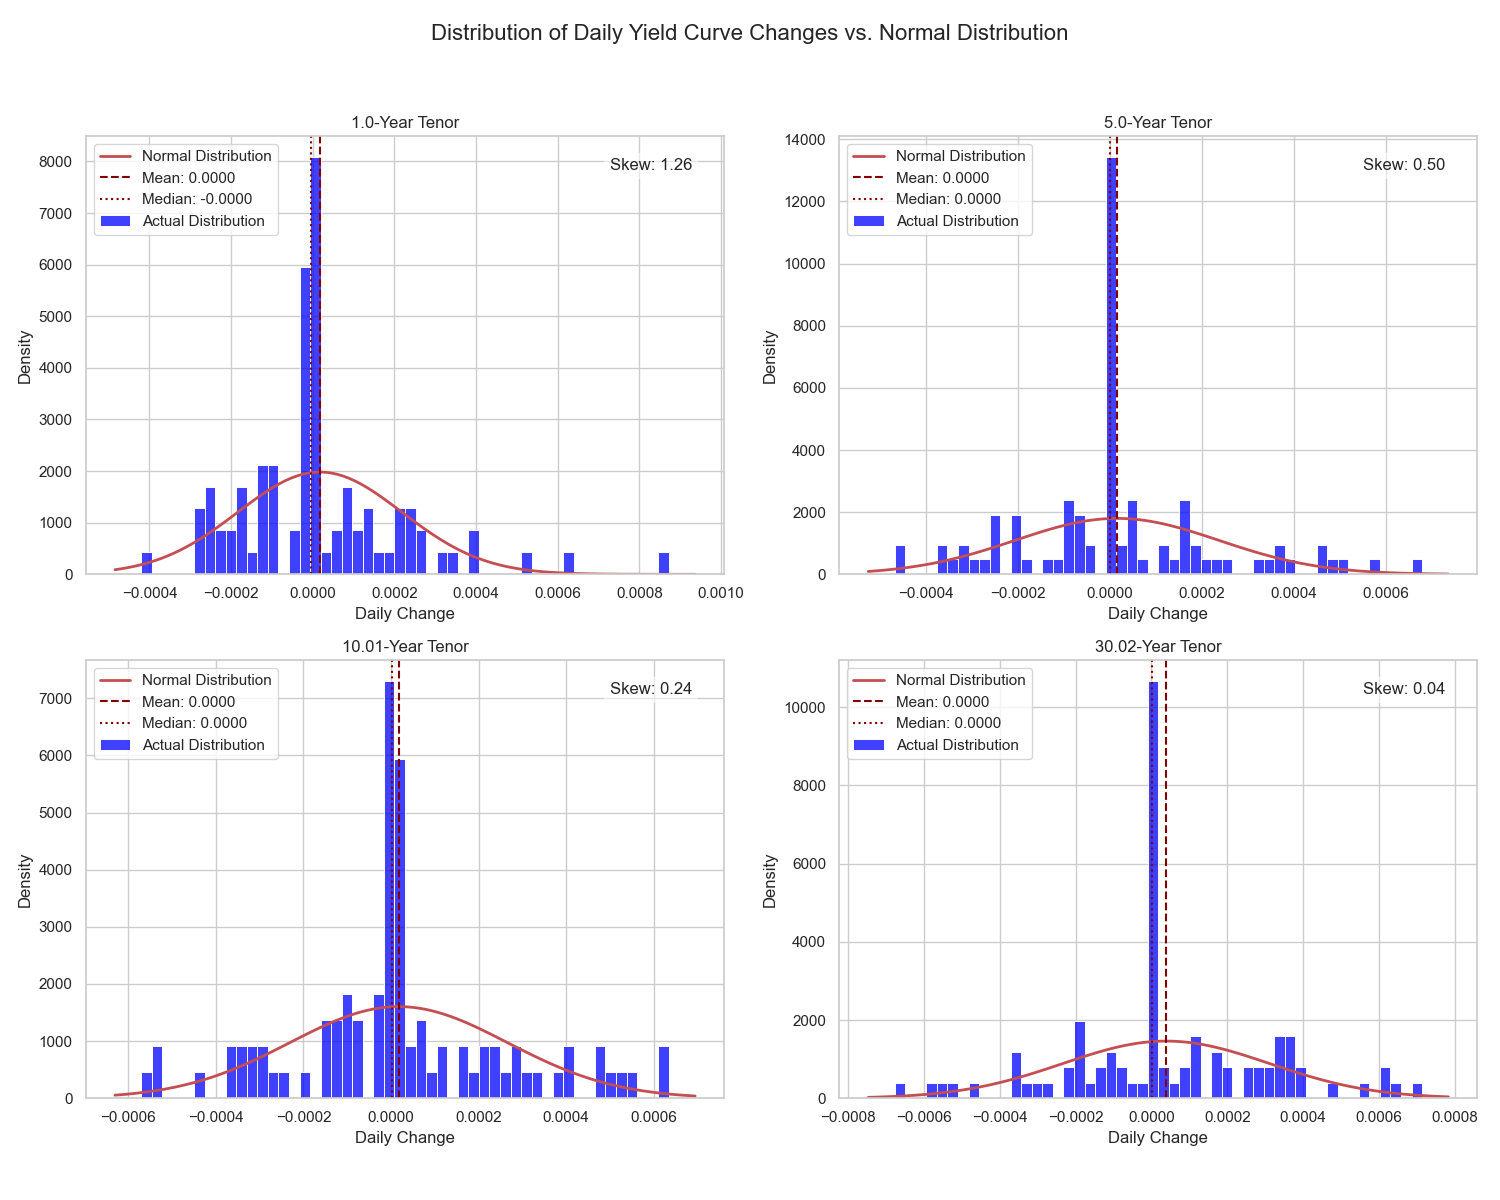
\includegraphics[width=1\textwidth]{images/descriptive_data_analysis/yield_curve_daily_changes_histogram.png}
	\caption{Histograms of Daily Yield Changes by Tenor}
	\label{fig:yield_curve_daily_changes_histogram}
\end{figure}

Figure~\ref{fig:yield_curve_daily_changes_histogram} compares empirical histograms of daily interest rate changes with theoretical normal distributions. All tenors display leptokurtic distributions with fat tails, implying that extreme movements occur more frequently than predicted by Gaussian models. The 1-year tenor exhibits pronounced positive skewness (1.26), suggesting a tendency toward larger upward rate movements. Skewness gradually declines for longer maturities. These findings confirm that interest rate changes deviate substantially from normality.

\begin{figure}[H]
	\centering
	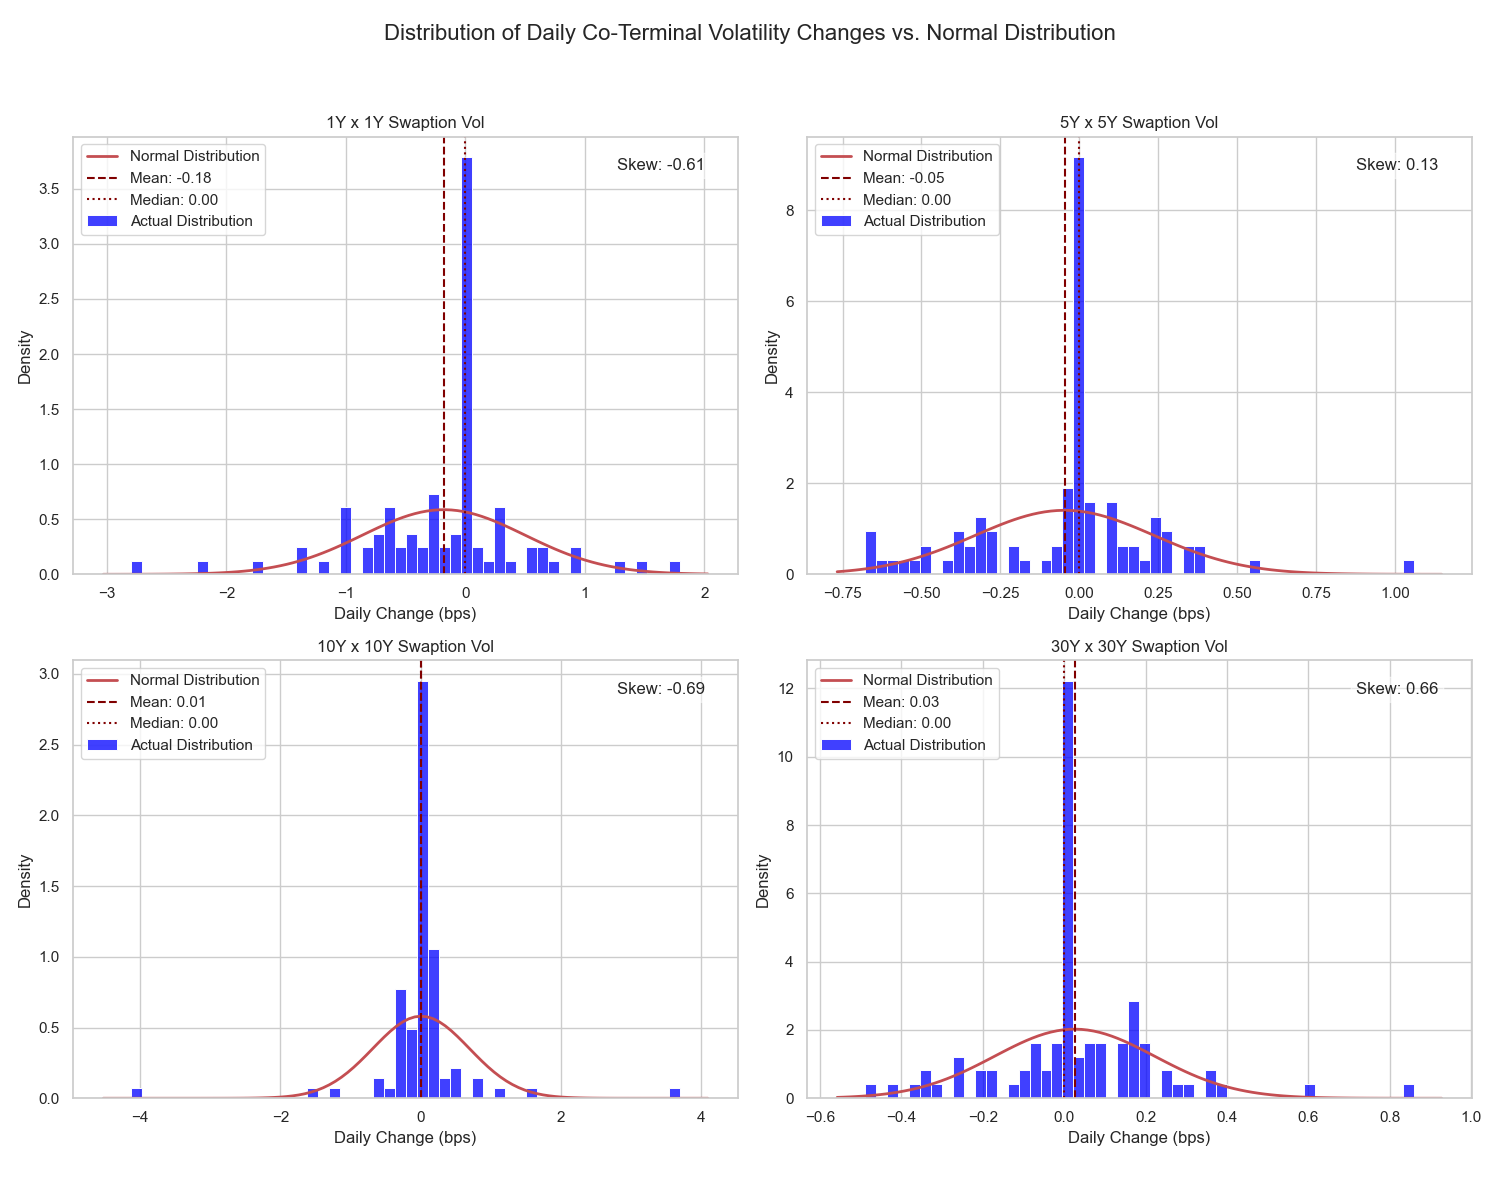
\includegraphics[width=1\textwidth]{images/descriptive_data_analysis/vol_surface_daily_changes_histogram.png}
	\caption{Histograms of Daily Swaption Volatility Changes}
	\label{fig:vol_surface_daily_changes_histogram}
\end{figure}

Figure~\ref{fig:vol_surface_daily_changes_histogram} presents the distribution of daily changes in swaption volatilities. Similar to yield changes, the data exhibit significant leptokurtosis and fat tails, confirming the non-normal nature of the underlying process. A mild positive skew is particularly evident in the 5-year tenor (skew = 0.50), indicating that large volatility spikes are more frequent than declines. Together with the findings from Figure~\ref{fig:yield_curve_daily_changes_histogram}, this evidence supports the use of non-parametric, data-driven models-such as \ac{nn}s-that can flexibly capture these empirical deviations from normality.

\subsection{Data Preprocessing}
\subsubsection{Bootstrapping Zero-Curves}
The implementation of the one-factor \ac{hw} model in \texttt{QuantLib} requires zero-coupon curves as input for both discounting and forward rate generation. Consequently, the \ac{eur} swap curves obtained from Bloomberg were bootstrapped into continuous zero rate term structures following the procedure outlined in section~\ref{subsec:bootstrap_zero_curve}. This ensures compatibility with the \texttt{QuantLib} framework and provides a consistent foundation for pricing swaptions and calibrating the model parameters.

\subsubsection{Handling Non-Trading Days in External Data}
The external market data obtained from Yahoo Finance, including the \ac{move} index, \ac{vix}, and EUR/USD exchange rate, is only available for trading days. In contrast, the swaption and swap curve datasets contain values for all calendar days, including weekends and public holidays. To ensure temporal consistency across all features used for \ac{hw} model calibration, the external data were reindexed to cover the entire daily date range of the analysis period.

Missing values corresponding to non-trading days were filled using a combination of forward-filling and backward-filling. Forward-filling propagates the most recent available value to subsequent missing days, while backward-filling assigns the nearest subsequent available value to preceding missing days. This procedure ensures that every day within the observation window has a corresponding value for each external variable, resulting in a continuous dataset that can be used by the \ac{nn} without introducing gaps or inconsistencies.

\subsubsection{Feature Engineering for the Neural Network}
In addition to the raw market data, several engineered features were created to enhance the \ac{nn}'s ability to predict \ac{hw} model parameters. These features capture the shape of the yield curve, relationships between external market indicators, and underlying latent structures via dimensionality reduction. Each feature was designed with a clear economic or statistical justification for its relevance to the model parameters: the volatility \(\sigma\) and the mean-reversion speed \(a\).

\paragraph{Features Engineered from the Yield Curve}
These features explicitly describe the shape and dynamics of the zero-coupon interest rate term structure. Let \(\text{Rate}(T)\) denote the zero-coupon rate for a given tenor \(T\) (e.g., \(\text{Rate}(10\text{Y})\) is the 10-year rate).

\textit{Slope Features:}
\begin{equation}
	\text{slope\_3m10y} = \text{Rate}(10\text{Y}) - \text{Rate}(3\text{M})
\end{equation}

\begin{equation}
	\text{slope\_2y10y} = \text{Rate}(10\text{Y}) - \text{Rate}(2\text{Y})
\end{equation}

\begin{equation}
	\text{slope\_5y30y} = \text{Rate}(30\text{Y}) - \text{Rate}(5\text{Y})
\end{equation}

A steep positive slope typically signals expectations of economic growth and future rate hikes, implying higher expected interest rate volatility (\(\sigma\)). Conversely, a flat or inverted curve suggests a more stable rate environment and lower \(\sigma\). Regarding mean reversion (\(a\)), a steep curve indicates strong anchoring to the long-term average, implying higher \(a\), while an inverted curve signals weaker anchoring and lower \(a\).

\textit{Curvature Features:}
\begin{equation}
	\text{curvature\_2y5y10y} = 2 \cdot \text{Rate}(5\text{Y}) - \text{Rate}(2\text{Y}) - \text{Rate}(10\text{Y})
\end{equation}

\begin{equation}
	\text{curvature\_1y2y5y} = 2 \cdot \text{Rate}(2\text{Y}) - \text{Rate}(1\text{Y}) - \text{Rate}(5\text{Y})
\end{equation}

\begin{equation}
	\text{curvature\_10y20y30y} = 2 \cdot \text{Rate}(20\text{Y}) - \text{Rate}(10\text{Y}) - \text{Rate}(30\text{Y})
\end{equation}

High curvature indicates significant uncertainty in medium-term rates, aiding prediction of the term structure of \(\sigma\). Pronounced curvature suggests rates are expected to revert to a mean, implying higher \(a\). Flat curvature indicates weaker mean reversion and lower \(a\).

\paragraph{Features Engineered from External Market Data} \mbox{}\\
\textit{Curvature-to-Slope Ratio:}
\begin{equation}
	\text{curvature\_slope\_ratio} = \frac{\text{curvature\_2y5y10y}}{\text{slope\_2y10y}}
\end{equation}
This feature captures nuanced market regimes where slope and curvature provide complementary information. It allows the network to distinguish between different economic environments and predict both \(\sigma\) and \(a\) more accurately.

\textit{\ac{move}-to-\ac{vix} Ratio:}
\begin{equation}
	\text{\ac{move}\_\ac{vix}\_Ratio} = \frac{\text{\ac{move}\_Open}}{\text{\ac{vix}\_Open}}
\end{equation}
A high ratio indicates stress concentrated in the bond market, signaling a higher \(\sigma\) specific to interest rates. It also implies uncertainty about central bank policy, potentially reducing \(a\). This feature helps the network separate general market panics from fixed-income-specific volatility.

\paragraph{Features Engineered via Dimensionality Reduction}
Instead of feeding all individual zero-coupon rates directly into the \ac{nn}, the yield curve was transformed using \ac{pca}. The reason for this choice lies in the fact that individual rates on the curve are highly correlated - a move in the 5-year rate is almost always accompanied by similar movements in the 7-year and 10-year rates as visible in figure \ref{fig:feature_correlation_prePCA}. Using these raw, correlated rates introduces several problems: multicollinearity, redundant information, and an increased risk of overfitting.

\begin{figure}[H]
	\centering
	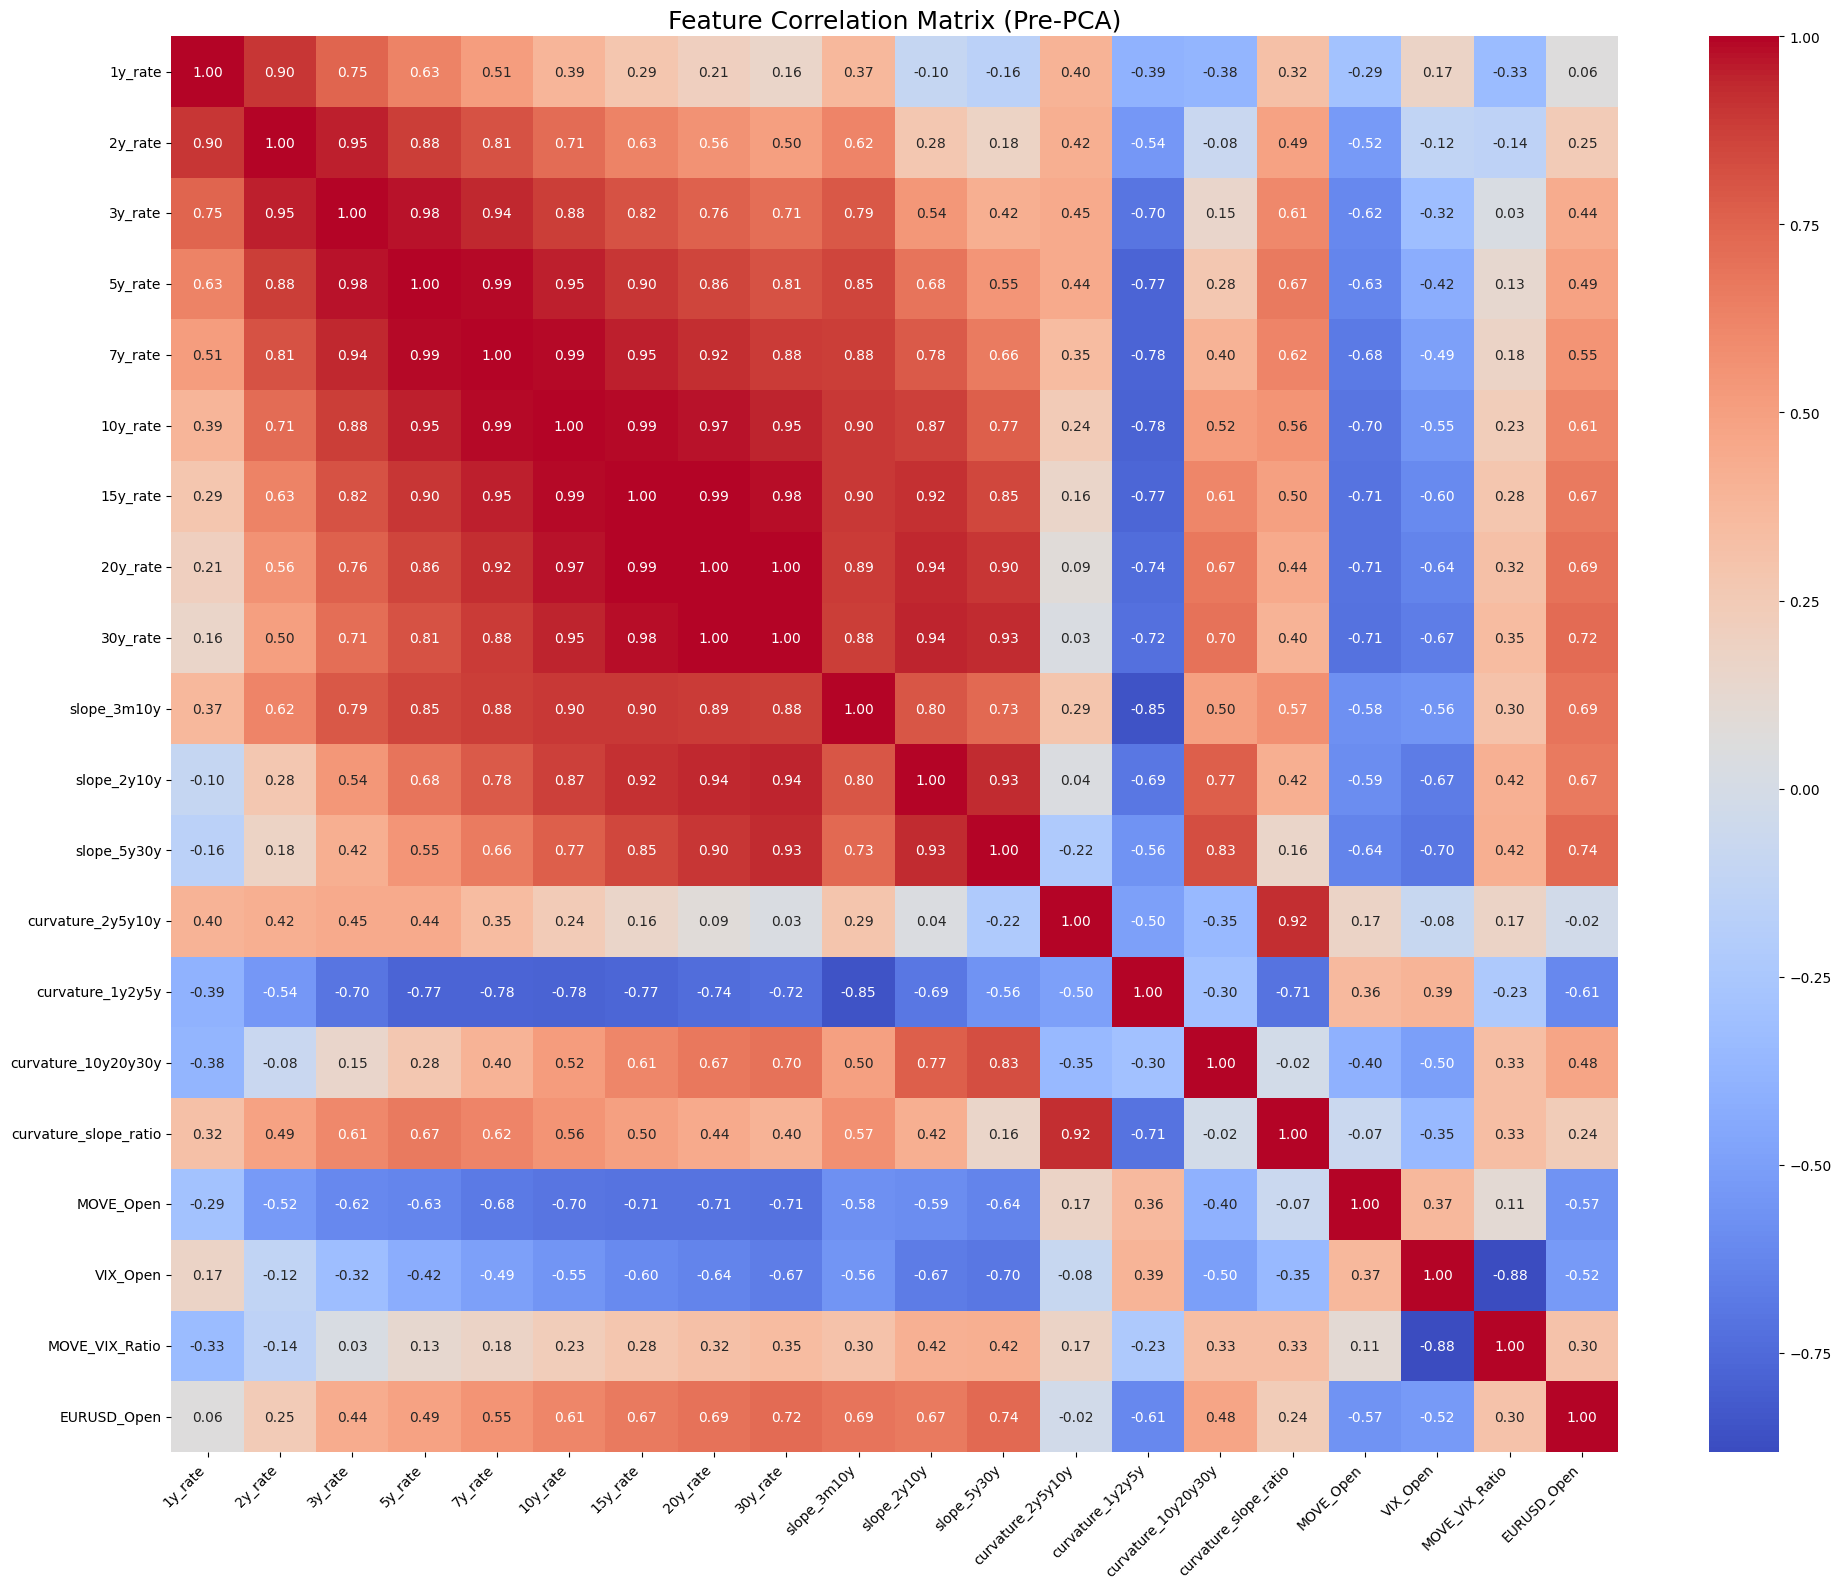
\includegraphics[width=1\textwidth]{images/features/feature_correlation_matrixPre-PCA.png}
	\caption{Correlation matrix of the engineered features before applying PCA.}
	\label{fig:feature_correlation_prePCA}
\end{figure}

Multicollinearity causes instability in the learned weights of the \ac{nn}. When input features contain overlapping information, the model struggles to assign stable importance to each feature. It may assign large, offsetting weights to features that move together, resulting in unstable and unreliable predictions \parencite[p.~2]{chan2022multicollinearity}.

Redundant information makes the learning process inefficient and typically leads to poor test performance \parencite[p.~3]{sildir2020redudantfeatures}. Most daily movements in the yield curve are dominated by a single pattern - a parallel shift. Feeding the model all the raw rates forces it to re-learn this shared structure repeatedly instead of focusing on economically meaningful dynamics such as slope or curvature changes.

High dimensionality further increases the complexity of the model, encouraging overfitting. With too many correlated features, the \ac{nn} risks memorizing noise instead of generalizable relationships, which harms out-of-sample performance \parencite[p.~3]{sildir2020redudantfeatures}.

\ac{pca} directly resolves these issues by transforming the vector of rates
\[
	R = [\text{Rate}(1\text{Y}), \text{Rate}(2\text{Y}), \dots, \text{Rate}(30\text{Y})]
\]
into a set of uncorrelated and economically interpretable components:
\begin{equation}
	\text{PC\_Level} = \mathbf{w}_1 \cdot \mathbf{R}
\end{equation}
\begin{equation}
	\text{PC\_Slope} = \mathbf{w}_2 \cdot \mathbf{R}
\end{equation}
\begin{equation}
	\text{PC\_Curvature} = \mathbf{w}_3 \cdot \mathbf{R}
\end{equation}

These three “super-features” capture nearly all the meaningful variation of the yield curve and can be interpreted as follows \parencite[pp.~98--107]{Rebonato_2018}:
\begin{itemize}
	\item PC\_Level represents the overall interest rate level and captures parallel shifts. Empirically, higher rate levels are associated with higher volatility (\(\sigma\)).
	\item PC\_Slope measures the steepness of the curve and reflects economic expectations, influencing both \(\sigma\) and \(a\).
	\item PC\_Curvature captures the non-linear “bow” of the curve, aiding the model in learning term-structure effects in the piecewise $\sigma$ and mean-reversion dynamics $\alpha$.
\end{itemize}

After applying \ac{pca} to the engineered features, the resulting correlation matrix exhibits a significant reduction in the highest correlations. The originally strong dependencies between individual yield curve rates and other features are largely removed as visible in figure \ref{fig:feature_correlation_postPCA}, demonstrating that the principal components provide a set of largely uncorrelated, independent features for the \ac{nn}.

\begin{figure}[H]
	\centering
	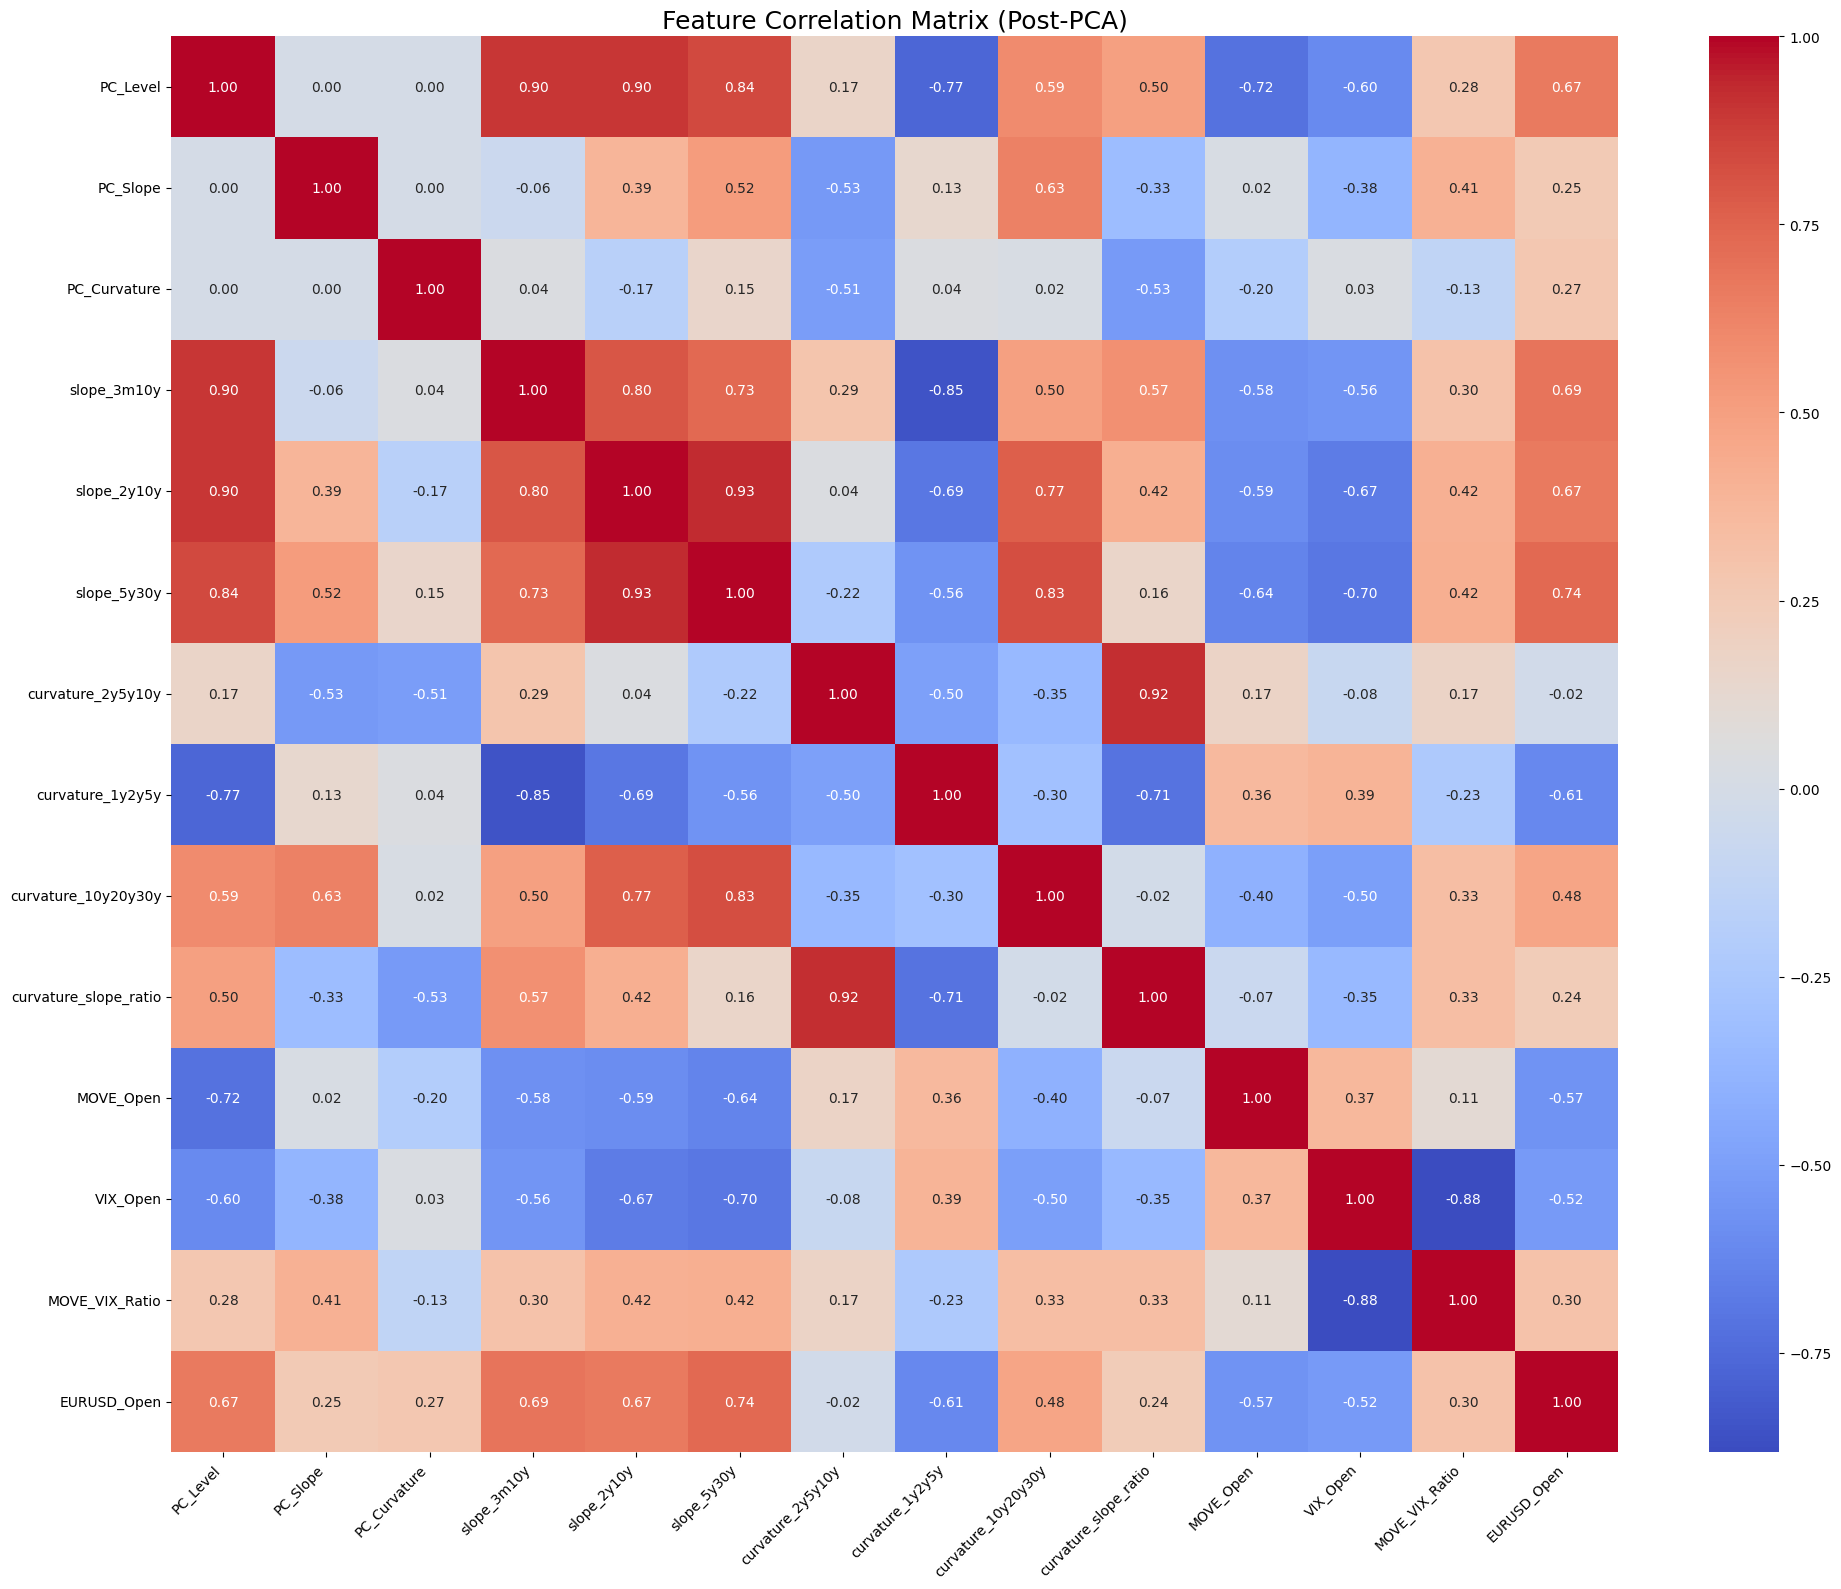
\includegraphics[width=1\textwidth]{images/features/feature_correlation_matrixPost-PCA.png}
	\caption{Correlation matrix of the engineered features after applying \ac{pca}.}
	\label{fig:feature_correlation_postPCA}
\end{figure}

By reducing the dimensionality from roughly ten correlated rate inputs to three independent components, \ac{pca} provides a stable, interpretable, and compact representation of the yield curve. This significantly improves the \ac{nn}'s training efficiency, robustness, and generalization performance.

\subsubsection{Feature Scaling}
Prior to being fed into the \ac{nn}, all input features are scaled using the \texttt{StandardScaler} from the \texttt{scikit-learn} library. This process, also known as standardization or Z-score normalization, ensures that each feature has a mean of zero and a standard deviation of one \parencite[pp.~31--32]{zheng2018feature}.

The scaling process consists of two main steps:

\textit{Step 1: Fit Phase (Learning from Training Data)}
The scaler analyzes the training data to learn the distribution of each feature. For each feature column, it calculates:

\begin{equation}
	\mu = \frac{1}{n} \sum_{i=1}^{n} x_i
\end{equation}
\begin{equation}
	\sigma = \sqrt{\frac{1}{n} \sum_{i=1}^{n} (x_i - \mu)^2}
\end{equation}

where \(x_i\) are the individual values of the feature and \(n\) is the number of training samples. The computed mean \(\mu\) and standard deviation \(\sigma\) are stored in the scaler object.

\textit{Step 2: Transform Phase (Applying the Scaling)}
The learned parameters are used to transform all values of that feature in the training, validation, and test datasets:

\begin{equation}
	z = \frac{x - \mu}{\sigma}
\end{equation}

This centers the data around zero and scales it to unit variance.

From a computational perspective, normalization is necessary to manage issues arising from the inherent structure of raw data inputs. It is a technique widely used in statistics for making the units of variables comparable, which is critical when input data are expressed in very different units and exhibit disparate orders of magnitude. Without scaling, features with very large numerical values can dominate the error calculation, causing the error reduction algorithm to focus primarily on these variables while neglecting the information contained in smaller-valued features. Furthermore, when raw numerical values are extremely large, such as on the order of $10^{6}$, their processing can generate outputs that exceed the capacity of standard computing hardware, making scaling essential to control for calculation and roundoff errors \parencite{shanker1996effectdatastandardization}.

The application of scaling directly addresses the optimization landscape of the training problem, leading to more efficient convergence. Normalizing the input is known to accelerate convergence during the optimization of linear models. Linear scale transformations, especially those that compress the search space, reduce the distance the backpropagation algorithm must cover in each iteration \parencite{sola1997importancedatanormalization}. This improved conditioning, where normalization helps ensure the covariance matrix of the layer input $\sum{}x$ is well-conditioned, is crucial for faster learning and aids the optimization algorithm in locating local minima \parencite{huang2020normalizationtechniquestrainingdnns}. Consequently, an adequate normalization protocol can significantly reduce calculation and training time, with studies showing that estimation errors can be reduced by a factor of 5 to 10 and the time required to achieve such results reduced by an order of magnitude \parencite{sola1997importancedatanormalization}.

Ultimately, the primary result of standardization is an improvement in the \ac{nn}'s quality and training stability. Data transformation is frequently used for improved learning, and normalization techniques are considered essential for accelerating the training and enhancing the generalization of deep \ac{nn}s. \ac{nn} trained on standardized data generally yield better overall results, leading to a higher classification rate and a smaller \ac{mse} in regression problems, where a smaller \ac{mse} indicates a higher quality solution \parencite{shanker1996effectdatastandardization}. The performance of a network, including the number of training iterations required and the final error attained, is enhanced as the input variable ranges are 'equalized' by the normalization process. This contributes to scale-invariant learning, which is important for stabilizing training and has been shown to be useful for adaptively adjusting the learning rate. In some cases, standardization is not merely a best practice but a formal prerequisite due to specific algorithm requirements \parencite{huang2020normalizationtechniquestrainingdnns}.

By applying \texttt{StandardScaler}, the \ac{nn} receives a well-conditioned, standardized input, which improves training stability, and convergence speed of the resulting model.

\subsection{Hyperparameter Optimization}
\label{subsec:hyperparameter_optimization}

The predictive performance and stability of \ac{nn}s depend critically on an appropriate choice of hyperparameters. To identify an optimal configuration, a structured hyperparameter optimization process was conducted using the Hyperband algorithm, as described in section~\ref{subsec:hyperband_algorithm}. This algorithm efficiently allocates computational resources to explore a broad hyperparameter space while focusing on the most promising configurations.

The core settings for the Hyperband tuner were configured as follows:
\begin{itemize}
	\item Maximum Epochs per Trial (\texttt{max\_epochs}): A total of 1,000 epochs were allocated as the maximum budget for training any single hyperparameter configuration.
	\item Reduction Factor (\texttt{factor}): A factor of 3 was used, meaning that after each round of training within a bracket, the number of configurations is reduced by a factor of 3, retaining only the top-performing third.
	\item Objective: The optimization objective was the minimization of the \ac{rmse} on the validation set.
\end{itemize}

The hyperparameters tuned in this study can be divided into two categories: those defining the \ac{nn} architecture and those related to the training process and loss function. Hyperparameters related to the architecture are:
\begin{itemize}
	\item Number of Hidden Layers: This parameter determines the depth of the \ac{nn}. A deeper \ac{nn} has greater representational power and can capture more complex nonlinear relationships in the data, but it also increases the risk of overfitting and computational cost. \newline
	      \textit{Search Space:} Integer between 1 and 5
	\item Number of Neurons per Layer: The width of each hidden layer, determined by the number of neurons, controls the capacity of the model. Larger layers allow for more detailed pattern recognition but can lead to overfitting if excessive. \newline
	      \textit{Search Space:} Integer between 16 and 128, in steps of 16, for each hidden layer
	\item The activation function introduces non-linearity into the \ac{nn}, enabling it to model complex relationships between input features and outputs. \newline
	      \textit{Search Space:} Choice between \texttt{\ac{relu}} and \texttt{\ac{tanh}}.
	\item Dropout is a regularization technique that randomly deactivates a fraction of neurons during training to prevent overfitting by discouraging co-adaptation among neurons. \newline
	      \textit{Search Space:} Boolean choice between \texttt{True} and \texttt{False}.
	\item Dropout Rate: If dropout is used, this parameter determines the fraction of neurons dropped during each training iteration. \newline
	      \textit{Search Space:} Floating-point value between 0.1 and 0.5 (only active if \texttt{use\_dropout = True}) in steps of 0.1.
\end{itemize}

Tuneable hyperparameters which cover the training and the loss functions are:
\begin{itemize}
	\item Learning Rate: The learning rate governs the step size used by the optimizer when updating the \ac{nn} weights. A high learning rate may lead to instability or divergence, whereas a very low one results in slow convergence. To capture effective values across orders of magnitude, the search was conducted on a logarithmic scale. \newline
	      \textit{Search Space:} Floating-point value between 0.0001 and 0.01, sampled logarithmically.

	\item Underestimation Penalty: This custom hyperparameter is designed to address the asymmetric cost of forecasting errors in financial volatility modeling. Underestimating volatility poses a greater financial risk than overestimating it. Therefore, this penalty increases the loss when the model underpredicts volatility, encouraging more conservative estimates. \newline
	      \textit{Search Space:} Floating-point value between 0.5 (penalty for overestimation) and 4.0 (strong penalty) in steps of 0.1.
\end{itemize}

\subsection{Loss Function and Error Metric}
\label{subsec:loss_function_and_error_metric}
The objective of the \ac{nn} is to determine the optimal set of weights $W$ and biases $b$ such that the predicted \ac{hw} parameters minimize the discrepancy between model-implied swaption volatilities and their market-observed counterparts. The \ac{nn} acts as a function
\begin{equation}
	\text{NN} : x \mapsto \theta(x; W, b),
\end{equation}
where $x \in \mathbb{R}^d$ is the input feature vector containing scaled and \ac{pca}-transformed market data (yield curve levels, slopes, curvatures, etc.) for a given day, and $\theta$ denotes the vector of \ac{hw} model parameters to be predicted. The \ac{nn} employs a residual architecture: instead of predicting $\theta$ directly, it predicts a deviation $\Delta z$ from a fixed initial guess $z_0$:
\begin{equation}
	\Delta z = \text{NN}(x; W, b), \quad
	z = z_0 + \Delta z.
\end{equation}
The predicted parameters are obtained by applying a scaled sigmoid to ensure they remain within a predefined range [0, U]:
\begin{equation}
	\theta(x; W, b) = U \cdot \sigma(z) = U \cdot \frac{1}{1 + e^{-z}}.
\end{equation}

The predicted parameters $\theta$ are subsequently used within the QuantLib library as a black-box function $V_{\text{QL}}$, which computes model-implied volatilities $\hat{\sigma}$ for a portfolio of $n$ swaptions given the additional market data $M_j$ on day $j$:
\begin{equation}
	\hat{\sigma} = V_{\text{QL}}(\theta, M_j) = \{\hat{\sigma}_1, \hat{\sigma}_2, \dots, \hat{\sigma}_n\}.
\end{equation}

The predictive accuracy of the network is quantified using the \ac{rmse}, which measures the average magnitude of deviation between model-implied and market-observed volatilities, expressed in \ac{bps}:
\begin{equation}
	\text{\ac{rmse}} = \sqrt{\frac{1}{n}\sum_{i=1}^{n}(\hat{\sigma}_i - \sigma_i)^2} \times 10000.
\end{equation}

\begin{table}[H]
	\centering
	\caption{Notation used in the \ac{rmse} formula}
	\begin{tabular}{lp{12cm}}
		\toprule
		Symbol           & Meaning                                                                                                                 \\
		\midrule
		$n$              & Total number of swaptions in the evaluation dataset                                                                     \\
		$\hat{\sigma}_i$ & Implied volatility predicted by the \ac{hw} model using the parameters generated by the \ac{nn} for the $i$-th swaption \\
		$\sigma_i$       & Market-observed implied volatility for the $i$-th swaption                                                              \\
		\bottomrule
	\end{tabular}
\end{table}

To align the optimization with practical calibration objectives, an asymmetric loss function is employed during training. For each day $j$, the loss is computed as the mean of weighted squared errors between predicted and observed volatilities:
\begin{equation}
	L_j(W, b) = \frac{1}{n} \sum_{i=1}^{n} w_i (\hat{\sigma}_i - \sigma_{j,i})^2,
\end{equation}
where the weight $w_i$ accounts for underestimation penalties:
\begin{equation}
	w_i =
	\begin{cases}
		P, & \text{if } \hat{\sigma}_i < \sigma_{j,i} \quad \text{(underestimation)},   \\
		1, & \text{if } \hat{\sigma}_i \geq \sigma_{j,i} \quad \text{(overestimation)}.
	\end{cases}
\end{equation}
Here, $P>1$ is the underestimation penalty, treated as a hyperparameter optimized using the Hyperband algorithm. This asymmetric weighting is applied exclusively during training to encourage conservative predictions, while evaluation on validation and test sets uses the standard (unweighted) \ac{rmse} to assess predictive accuracy objectively.

The overall training objective is to identify network parameters $(W^*, b^*)$ that minimize the expected daily loss over the distribution of training data $D$:
\begin{equation}
	(W^*, b^*) = \arg \min_{W, b} \ \mathbb{E}_{(x_j, \sigma_j, M_j) \sim D} \left[ L_j(W, b) \right].
\end{equation}
In practice, this expectation is approximated by iterating over the training set day by day (batches) using the stochastic optimizer Adam:
\begin{equation}
	W_{t+1} = W_t - \eta \nabla_W L_j(W_t, b_t),
\end{equation}
where $\eta$ is the learning rate. Since $V_{\text{QL}}$ is a non-differentiable black-box function, gradients are computed numerically via finite differences using a tf.custom\_gradient implementation.

\subsection{Conversion from Normal to Black Volatility Errors}
\label{subsec:conversion_from_normal_to_lognormal_errors}
In interest rate derivatives markets, two primary volatility conventions are employed for pricing and risk management: the normal (Bachelier) volatility and the lognormal (Black) volatility. The distinction between these conventions arises from the assumed stochastic dynamics of the underlying forward rate or price process. The conversion between both representations is essential when comparing model calibration errors or implied volatilities expressed under different modeling assumptions, as is the case in the present study.

Under the Bachelier (normal) model, the forward rate \( F_t \) evolves according to a normal diffusion process,
\begin{equation}
	dF_t = \sigma_N \, dW_t,
\end{equation}
where \( \sigma_N \) denotes the normal volatility and \( W_t \) is a standard Brownian motion. In this framework, the forward rate can take both positive and negative values, making the model particularly suitable for low or negative interest rate environments. The option price under the Bachelier model is linear in volatility, and \( \sigma_N \) represents an absolute volatility level (for example, 0.0050 corresponds to 50 \ac{bps}).

In contrast, the Black (lognormal) model assumes that the forward rate follows a lognormal diffusion process,
\begin{equation}
	dF_t = \sigma_B F_t \, dW_t,
\end{equation}
where \( \sigma_B \) represents the lognormal or Black volatility. Here, the volatility is expressed in relative terms (e.g., 0.20 corresponds to 20\%), and the forward rate is strictly positive. The lognormal assumption is particularly useful when modeling multiplicative dynamics in markets with positive rates.

For \ac{atm} swaptions, where the strike \( K \) equals the forward rate \( F \), the two pricing frameworks yield nearly equivalent option values if the volatilities satisfy the following approximate relationship \parencite{hagan2002managingsmilerisk}:
\begin{equation}
	\sigma_N \approx \sigma_B F.
\end{equation}
Rearranging this yields an approximation for converting normal volatility to lognormal volatility:
\begin{equation}
	\sigma_B \approx \frac{\sigma_N}{F}.
\end{equation}
This relationship provides an accurate first-order approximation for \ac{atm} instruments and is commonly applied in market practice for fast conversions between volatility conventions.

When assessing model calibration performance, the model error expressed in normal volatility terms, denoted by \( \varepsilon_N \), can therefore be converted into an equivalent Black volatility error for each swaption \( i \) with forward rate \( F_i \) as
\begin{equation}
	\varepsilon_{B,i} = \frac{\varepsilon_N}{F_i}.
\end{equation}
This conversion enables a consistent comparison with benchmark results, such as those reported in studies or market data expressed in Black volatility terms.

However, aggregating these individual instrument errors to obtain a portfolio-level measure requires careful consideration. A simple average of volatility errors, while statistically valid, would be financially naive, as it assumes that a one-basis-point error has the same significance for every swaption. In practice, the financial impact of a volatility misestimation varies dramatically across instruments, depending on their sensitivity to volatility.

This sensitivity is precisely quantified by the instrument's vega. As established in foundational derivatives literature, the first-order approximation for the change in an option's price (\(\Delta V\)) due to a change in volatility (\(\Delta \sigma\)) is given by the relationship \( \Delta V \approx \nu \cdot \Delta \sigma \) \parencite[pp.~415-417]{hull2015optionsfutures}. In the context of this analysis, the model's normal volatility error, \( \varepsilon_N \), represents the \( \Delta \sigma \) term. Consequently, the pricing error, or P\&L impact, for a given swaption \( i \) is approximately \( \nu_i \cdot \varepsilon_N \). The vega for swaption \( i \) is formally defined as:
\begin{equation}
	\nu_i = \frac{\partial V_i}{\partial \sigma_N}.
\end{equation}
In the present context, vegas are computed under the Bachelier model, consistent with the representation of the input errors in normal volatility terms. The scientific rationale for weighting individual errors by vega is grounded in the fundamental principles of differential calculus as applied to derivative pricing. A model's error in the volatility dimension, \(\varepsilon_N\), does not translate uniformly to pricing error across all instruments. Instead, the first-order approximation of the pricing error, \(\Delta V\), is directly proportional to the volatility error, scaled by the instrument's vega: \( \Delta V \approx \nu \cdot \varepsilon_N \).

Vega therefore acts as a linear sensitivity coefficient, converting an abstract error measured in basis points of volatility into a tangible error measured in monetary units. An unweighted average of volatility errors would be statistically valid but financially naive, as it would implicitly assume that a one-basis-point error on a swaption with high vega has the same financial significance as the same error on a swaption with low vega. To construct a portfolio-level error metric that accurately reflects the aggregate financial impact of individual mispricings, it is therefore necessary to weight each volatility error by its corresponding vega. This ensures the resulting metric moves beyond a simple statistical average to provide a more robust and financially meaningful assessment of the model's performance, which is essential for its utility in risk management and hedging.

Using the swaption vegas as weighting factors is the direct implementation of this principle. To obtain a single, representative portfolio-level Black volatility error, a vega-weighted average is computed across all \( n \) swaptions. This ensures that instruments with a higher price sensitivity to volatility contribute proportionally more to the aggregate measure. The aggregated Black volatility error \( \bar{\varepsilon}_B \) is given by:
\begin{equation}
	\bar{\varepsilon}_B = \frac{\sum_{i=1}^{n} \varepsilon_{B,i} \nu_i}{\sum_{i=1}^{n} \nu_i}.
\end{equation}
Substituting the expression for \( \varepsilon_{B,i} \) yields:
\begin{equation}
	\bar{\varepsilon}_B = \frac{\sum_{i=1}^{n} \left( \frac{\varepsilon_N}{F_i} \nu_i \right)}{\sum_{i=1}^{n} \nu_i}.
\end{equation}
Since the normal-volatility-based model error \( \varepsilon_N \) is constant across swaptions on a given day, it can be factored out:
\begin{equation}
	\bar{\varepsilon}_B = \varepsilon_N \frac{\sum_{i=1}^{n} \frac{\nu_i}{F_i}}{\sum_{i=1}^{n} \nu_i}.
\end{equation}
This formula represents the vega-weighted average conversion from normal to lognormal volatility on the portfolio level. Conceptually, this approach yields a portfolio-consistent transformation of model errors that is grounded in financial reality, allowing for a robust comparison of calibration quality under different modeling frameworks.

Having established the framework for converting and aggregating calibration errors into a financially sound, portfolio-level metric, the following section describes the specific calibration strategy employed.

\subsection{Calibration Strategy}
The calibration methodology implemented in this thesis aligns with the \textit{simultaneous optimization} strategy discussed in section \ref{calibration}. The \ac{nn} is configured to concurrently optimize all dynamic parameters of the \ac{hw} model within a single, unified optimization routine.

Specifically, the approach treats the mean-reversion parameter, $\alpha$, as a single constant value and the volatility parameter, $\sigma(t)$, as a piecewise-constant function with seven distinct time segments. The \ac{nn}'s output layer predicts the complete set of these eight parameters. During the training loop, the custom gradient calculation within the \texttt{\_perform\_training\_step} function computes the gradients of the loss function with respect to all eight parameters simultaneously. The optimizer then updates all model weights to jointly minimize the pricing error (\ac{rmse}), thereby fitting both $\alpha$ and $\sigma(t)$ at the same time. This is in contrast to a two-step approach where parameters are estimated sequentially or a fixed mean-reversion approach where $\alpha$ is not optimized at all.

Furthermore, the calibration employs a \textit{global (full matrix) calibration} methodology with the exception of swaptions which have a maturity and tenor of less than 2 years. This global approach provides the model with a comprehensive view of the market, enabling it to achieve a more robust and stable fit across the entire volatility surface, as recommended for empirical analyses in section \ref{calibration}.

The following section outlines the experimental framework established to compare the performance of the \ac{nn} predictor against the traditional \ac{lm} optimization method.

\subsection{Comparison of Neural Network and Levenberg-Marquardt Calibration}
\label{subsec:comparison_of_nn_and_lm}
A robust experimental framework was designed to enable a scientifically valid comparison between the \ac{nn} predictor and the traditional \ac{lm} optimization. Recognizing that the performance of iterative optimizers can be highly dependent on their starting conditions, the \ac{lm} algorithm was implemented under three distinct initial guess strategies. The primary objective of this framework was to address the methodological challenge of fairly comparing an out-of-sample predictor against several variations of an in-sample fitter.

The core issue arises from the differing nature of the two model types. The \ac{lm} algorithm operates as an in-sample fitter: for a given day, it receives a set of market-observed swaption volatilities and determines the \ac{hw} parameters $(a, \sigma)$ that minimize the pricing error for this exact set. This approach can be prone to overfitting, as the resulting parameters may capture noise specific to the input data. In contrast, the \ac{nn} is designed as an out-of-sample predictor, trained on historical data to learn a mapping from observable market features to the optimal \ac{hw} parameters, making its error an inherent measure of generalization ability. This distinction is fundamental because the ultimate purpose of any model calibration extends beyond mere in-sample fitting. While an optimizer's primary function is to achieve a minimal error on a given set of instruments, its practical utility is defined by its ability to derive parameters that accurately represent the underlying market dynamics. Consequently, a successful calibration must yield parameters capable of consistently pricing related financial instruments beyond the immediate calibration set. The \textit{Intra-Day Hold-Out Set} framework is explicitly designed to quantify this precise generalization capability. Therefore, this comparison does not contest the \ac{lm} algorithm's efficacy as a pure curve-fitting tool. Instead, it provides a rigorous assessment of each method's ability to produce robust, generalizable parameters suitable for broader applications in pricing and risk management, which is the essential, albeit implicit, requirement for any robust calibration tool.

To reconcile this methodological inconsistency, an \emph{Intra-Day Hold-Out Set} framework was employed. This protocol enforces a uniform out-of-sample evaluation for all models. Each day within the test period was processed as follows. First, all valid swaptions were assembled and partitioned into calibration and hold-out sets using stratified random sampling, with the swaption expiry date as the stratification variable. Within each expiry stratum, 80\% of the instruments were assigned to the calibration set and the remaining 20\% to the hold-out set. This partitioned data was then used to calibrate not one, but three distinct variations of the \ac{lm} optimizer, each designed to test a different hypothesis regarding the optimal handling of initial parameter guesses in a time-series context.

Once the data partitioning was completed, all models generated their \ac{hw} parameters. The pre-trained \ac{nn} produced its parameters via a single forward pass using only the day's market features. In parallel, the three \ac{lm} strategies were calibrated using only the 80\% calibration set. The first, termed the 'Static Cold Start,' served as the scientific baseline, utilizing a fixed initial guess for every day of the test period to ensure a stable and reproducible performance reference. The second, the 'Pure Rolling Warm Start,' was designed to test a common heuristic by using its own calibrated parameters from day $t-1$ as the initial guess for day $t$, thereby allowing for an investigation into the risks of error propagation and parameter drift. The third and most sophisticated approach, the 'Adaptive Anchor,' was developed as a robust solution to the challenges of parameter drift and market regime shifts. This strategy creates its initial guess, $\theta_{t}^{\text{guess}}$, for day $t$ from a dynamic, error-based weighted average of its own calibrated parameters from the previous day, $\theta_{t-1}^{\text{adaptive}}$, and the stable static anchor, $\theta^{\text{static}}$. This design manages the trade-off between exploiting recent market information and exploring from a known-good baseline. The core of this strategy is the dynamic weight, $w_t$, which adjusts the model's reliance on the previous day's result based on its historical performance. The weight is calculated on each day prior to calibration using a linear interpolation function that maps the previous day's out-of-sample \ac{rmse}, denoted $\text{RMSE}_{t-1}$, to a trust level.

Specifically, the dynamic weight $w_t$ is determined by first scaling the error to a normalized range $[0, 1]$ and then interpolating between a predefined maximum and minimum trust level. The scaled error, $e_t^{\text{scaled}}$, is computed as:
\begin{equation}
	e_t^{\text{scaled}} = \text{max}\left(0, \text{min}\left(1, \frac{\text{RMSE}_{t-1} - \text{RMSE}_{\text{min}}}{\text{RMSE}_{\text{max}} - \text{RMSE}_{\text{min}}}\right)\right)
\end{equation}
where $\text{RMSE}_{\text{min}}$ and $\text{RMSE}_{\text{max}}$ are predefined thresholds for good and poor performance, respectively. The weight $w_t$ is then calculated to have an inverse relationship with this scaled error:
\begin{equation}
	w_t = w_{\text{max}} - e_t^{\text{scaled}} \cdot (w_{\text{max}} - w_{\text{min}})
\end{equation}

In this framework, $w_{\text{max}}$ represents the maximum trust in the rolling guess during periods of stability, while $w_{\text{min}}$ enforces a strong reversion to the static anchor during periods of high error. For this study, the hyperparameters were set to $\text{RMSE}_{\text{min}} = 6.0$ bps, $\text{RMSE}_{\text{max}} = 12.0$ bps, $w_{\text{max}} = 0.95$, and $w_{\text{min}} = 0.15$. This mechanism ensures that the model automatically becomes more conservative in volatile markets and more aggressive in stable, trending markets.

The efficacy of the \ac{lm} strategies is fundamentally dependent on the quality of the baseline initial guess that serves as their stable anchor. To ensure this anchor was robust and represented a globally sensible starting point, it was determined through a computationally intensive pre-computation step, separate from the main testing phase. A genetic algorithm, specifically employing a general island model approach, was utilized for this purpose. This global optimization technique is particularly well-suited for exploring the complex, non-convex error surface of the calibration problem, mitigating the risk of selecting an initial guess from a suboptimal local minimum (see \ref{subsec:generalized_island_model}). The algorithm was run on the full swaption volatility surface from 03.08.2025, the day immediately preceding the start of the test period. To focus on the more liquid and significant instruments, swaptions with either a tenor or a maturity of less than two years were excluded from this initial calculation. The resulting parameter set, detailed in table \ref{tab:initial_guess}, was then used as the fixed initial guess throughout the subsequent experiment.

\begin{table}[H]
	\centering
	\begin{threeparttable}
		\caption{Initial Guess for Levenberg-Marquardt Strategies}
		\label{tab:initial_guess}
		\begin{tabular}{ll}
			\toprule
			Parameter  & Initial Value          \\
			\midrule
			$\alpha$   & 0.01821630830602023    \\
			\addlinespace
			$\sigma_1$ & 0.00021102917641460398 \\
			$\sigma_2$ & 0.00026161313022069355 \\
			$\sigma_3$ & 0.0002433782032732618  \\
			$\sigma_4$ & 0.00023207666803595517 \\
			$\sigma_5$ & 0.00019547828248440554 \\
			$\sigma_6$ & 0.00013296374054782453 \\
			$\sigma_7$ & 0.0001745673951321553  \\
			\bottomrule
		\end{tabular}
		\begin{tablenotes}
			\item \footnotesize Note: The parameter values were determined as a one-off pre-computation using a Genetic Algorithm (Island Model) on a representative dataset prior to the testing period.
		\end{tablenotes}
	\end{threeparttable}
\end{table}

In contrast to the iterative LM methods, the \ac{nn} architecture also incorporates an initial parameter guess, but for a fundamentally different purpose. The network is designed as a residual model, meaning it does not predict the absolute parameter values directly. Instead, it learns to predict a correction, $\Delta \theta_{\text{predicted}}$, to a predefined baseline, $\theta_{\text{initial}}$. The final parameter estimate is then constructed as their sum:
\begin{equation}
	\theta_{\text{final}} = \theta_{\text{initial}} + \Delta \theta_{\text{predicted}}
\end{equation}
This residual formulation simplifies the learning task, as the \ac{nn} only needs to approximate local adjustments rather than the entire complex mapping from market features to parameters, which empirically leads to faster convergence and improved stability.

The choice of this baseline, $\theta_{\text{initial}}$, is flexible; it can be derived from various sources, such as parameters from the previous trading day or a traditional calibration. For this study, to provide a consistent and stable reference point, the initial guess was determined by calibrating the \ac{hw} model on the first day of the training set using the \ac{lm} algorithm. The resulting parameters were then rounded to create a generalized, central reference point. This rounding discourages the network from merely replicating the specific local minimum found by the initial \ac{lm} calibration and encourages it to learn a more robust mapping. The fixed values used as this baseline for the \ac{nn}'s residual predictions throughout the study are detailed in table \ref{tab:nn_initial_guess}.

\begin{table}[H]
	\centering
	\begin{threeparttable}
		\caption{Initial Guess Baseline for the Residual Neural Network}
		\label{tab:nn_initial_guess}
		\begin{tabular}{l c}
			\toprule
			Parameter  & Initial Guess Value \\
			\midrule
			$\alpha$   & 0.02000             \\
			\addlinespace
			$\sigma_1$ & 0.00020             \\
			$\sigma_2$ & 0.00020             \\
			$\sigma_3$ & 0.00017             \\
			$\sigma_4$ & 0.00017             \\
			$\sigma_5$ & 0.00017             \\
			$\sigma_6$ & 0.00017             \\
			$\sigma_7$ & 0.00017             \\
			\bottomrule
		\end{tabular}
		\begin{tablenotes}
			\item \footnotesize Note: Values were determined via an \ac{lm} calibration on the first day of the training set and subsequently rounded.
		\end{tablenotes}
	\end{threeparttable}
\end{table}

Finally, the parameters generated by the \ac{nn} and all three \ac{lm} strategies were evaluated on the identical 20\% hold-out set and the required calibration time was measured. Each model was used to price the hold-out swaptions, and the \ac{rmse} between model-implied volatilities and observed market volatilities was computed. This uniform evaluation enabled a direct and fair comparison of the models' relative generalization power in unseen market conditions.

\subsection{Methodological Workflow Summary}
The end-to-end analytical framework commences with the acquisition of the dataset, which is temporally partitioned into distinct training, validation, and test sets to ensure a rigorous evaluation of model generalization. The raw data subsequently undergoes a multi-stage preprocessing pipeline designed to extract salient features and prepare the inputs for modeling. This pipeline begins with the bootstrapping of raw swap rates to construct continuous zero-coupon yield curves, a prerequisite for the QuantLib pricing engine. Concurrently, external market data is temporally aligned with the primary dataset by resampling to a daily frequency and imputing values for non-trading days. A sophisticated feature engineering process is then applied, creating variables that describe the yield curve's shape, such as slope and curvature, alongside engineered indicators like the MOVE-to-VIX ratio. To mitigate multicollinearity and reduce dimensionality, Principal Component Analysis is performed on the yield curve rates, distilling their dynamics into three orthogonal factors representing level, slope, and curvature. Finally, all engineered features are standardized using a Z-score scaler, which is fitted exclusively on the training data to prevent data leakage.

With the data prepared, the \ac{nn} model is developed. An optimal \ac{nn} architecture and its associated hyperparameters are identified through a systematic search using the Hyperband algorithm, with performance assessed on the validation set. The final model, which employs a residual architecture to predict corrections to a baseline parameter set, is then trained on the complete training dataset. In parallel, the benchmark \ac{lm} optimizer is prepared for the final comparison. A critical pre-computation step is executed to establish a robust initial parameter guess, which serves as a stable anchor for the iterative optimizations. This is achieved by running a global optimization via a genetic algorithm on the full swaption volatility surface from the day immediately preceding the test period.

The final stage consists of a direct, out-of-sample comparison conducted daily on the test set. For each day, an "Intra-Day Hold-Out Set" protocol is implemented, partitioning the day's swaptions into an 80\% calibration set and a 20\% hold-out set. The trained \ac{nn} generates its parameters through a single forward pass based on the day's market features, scaled with the scaler fitted to the training data. Simultaneously, the \ac{lm} algorithm is calibrated using only the 80\% calibration set. The parameters generated by both methods are then used to price the swaptions in the 20\% hold-out set. The generalization performance of each model is quantified by the Root Mean Squared Error between the model-implied and market-observed volatilities, facilitating a direct and unbiased comparison of their predictive capabilities.

Following the execution of the comparative evaluation framework, a further series of analyses were conducted to facilitate a deeper interpretation of the model's behavior and to present the empirical findings comprehensively. To elucidate the internal decision-making process of the \ac{nn}, the final trained model was subjected to an interpretability analysis using \ac{shap}. This post-hoc analysis quantifies the marginal contribution of each input feature to the model's predictions, thereby rendering the behavior of the otherwise opaque model transparent. The resulting SHAP value plots provide crucial insights into the learned relationships between market drivers and the calibrated model parameters. In parallel, the daily performance metrics and parameter outputs generated during the evaluation phase were systematically aggregated. This data serves as the foundation for the creation of all subsequent visualizations, including time-series plots of model errors and parameter stability. Furthermore, these aggregated results were exported to CSV files to ensure reproducibility and to facilitate the direct construction of the summary tables presented in the empirical results section of this thesis.

% Define custom colors inspired by Matplotlib's "coolwarm"
\definecolor{coolcolor}{RGB}{103, 132, 180}
\definecolor{warmcolor}{RGB}{212, 98, 98}
\begin{figure}[H]
	\centering
	\begin{tikzpicture}[
			scale=0.75, transform shape,
			% Node Styles
			block/.style={rectangle, draw, fill=warmcolor!40, text width=9em, text centered, rounded corners, minimum height=4em},
			line/.style={draw, -Latex},
			cloud/.style={ellipse, draw, fill=coolcolor!30, minimum height=2em, text width=7em, text centered},
			process/.style={rectangle, draw, fill=warmcolor!30, text width=10em, text centered, rounded corners, minimum height=4em},
			io/.style={trapezium, trapezium left angle=70, trapezium right angle=110, draw, fill=coolcolor!30, text centered, minimum height=3em, text width=8em},
			comment/.style={rectangle, draw, dashed, fill=gray!15, text width=11em},
			% Style for the fitting dashed box
			fit-box/.style={draw, dashed, rounded corners, inner sep=0.4cm}
		]

		% == NODES ==
		% --- Top Section ---
		\node[cloud] (start) {Raw Market Data (Swaptions, Curves, Indicators)};
		\node[process, below=1cm of start] (split) {Temporal Split: Training, Validation, and Test Sets};
		\node[process, below=1cm of split] (preprocess) {Preprocessing Pipeline (Fit on Training Data)};
		\node[comment, right=0.5cm of preprocess] (preprocess-comment) {\textit{Includes:} \\ Bootstrapping, Feature Engineering, PCA, Standardization};

		% --- Offline Phases (Left and Right Branches) ---
		\node[process, below=1.2cm of preprocess, xshift=-5.5cm] (nn-train) {NN Hyperparameter Tuning \& Training (on Train/Val Sets)};
		\node[io, below=0.8cm of nn-train] (nn-model) {Trained NN Model};

		\node[process, below=1.2cm of preprocess, xshift=5.5cm] (lm-setup) {LM Initial Guess Determination (Genetic Algorithm on data from T-1)};
		\node[io, below=0.8cm of lm-setup] (lm-guess) {LM Initial Guess};

		% --- Daily Evaluation Loop (Central Flow) ---
		\node[block, below=1cm of $(nn-model.south)!0.5!(lm-guess.south)$] (daily-loop) {Daily Comparative Evaluation Loop (on Test Set)};
		\node[process, below=1cm of daily-loop] (intra-day-split) {Intra-Day Split: 80\% Calibration Set \& 20\% Hold-Out Set};
		\node[process, below=1cm of intra-day-split, xshift=-4.5cm, text width=7em] (nn-predict) {NN Prediction (Forward Pass)};
		\node[process, below=1cm of intra-day-split, xshift=4.5cm, text width=8em] (lm-calibrate) {LM Calibration (on 80\% Calibration Set)};
		\node[io, below=0.8cm of nn-predict] (nn-params) {NN HW Parameters};
		\node[io, below=0.8cm of lm-calibrate] (lm-params) {LM HW Parameters};
		\node[process, below=0.8cm of $(nn-params.south)!0.5!(lm-params.south)$] (evaluate) {Evaluate both parameter sets on 20\% Hold-Out Set};
		\node[io, below=0.8cm of evaluate, text width=12em] (results) {Out-of-Sample RMSE (Unweighted \& Vega-Weighted)};
		\node[block, below=0.8cm of results, fill=warmcolor!50] (compare) {Performance Comparison};

		% == ARROWS & CONNECTIONS ==
		\path [line] (start) -- (split);
		\path [line] (split) -- (preprocess);
		\path [line] (preprocess) -- (nn-train);
		\path [line] (preprocess) -- (lm-setup);
		\path [line] (nn-train) -- (nn-model);
		\path [line] (lm-setup) -- (lm-guess);
		\path [line, dashed] (split.east) -| ++(7,0) |- (daily-loop.north);
		\path [line] (daily-loop) -- (intra-day-split);
		\path [line] (intra-day-split) -- (nn-predict);
		\path [line] (intra-day-split) -- (lm-calibrate);
		\path [line] (nn-model) -- (nn-predict);
		\path [line] (lm-guess) -- (lm-calibrate);
		\path [line] (nn-predict) -- (nn-params);
		\path [line] (lm-calibrate) -- (lm-params);
		\path [line] (nn-params) -- (evaluate);
		\path [line] (lm-params) -- (evaluate);
		\path [line] (evaluate) -- (results);
		\path [line] (results) -- (compare);
		\path [draw, dashed] (preprocess.east) -- (preprocess-comment.west);

		% == Dashed boxes for Offline Phases using FIT library ==
		% This must be done AFTER the nodes to be fitted are defined.
		\node[fit-box, fit=(nn-train) (nn-model), label={[text=warmcolor!80!black]above:Offline NN Phase}] {};
		\node[fit-box, fit=(lm-setup) (lm-guess), label={[text=warmcolor!80!black]above:Offline LM Phase}] {};

	\end{tikzpicture}
	\caption{The end-to-end methodological workflow, from data preparation and model training to the final daily out-of-sample comparative evaluation.}
	\label{fig:workflow_chart}
\end{figure}

\subsection{Technical Setup and Computational Framework}
\label{subsec:technical_setup}
The implementation of the \ac{nn}-based \ac{hw} calibration framework was carried out in Python 3.12.3, employing TensorFlow 2.15 for the \ac{nn} architecture and QuantLib 1.34 for the financial modeling components. All experiments were conducted on a commercially available laptop equipped with an AMD~Ryzen~7~7840HS (\~ 3.8~GHz) processor with 16 cores.

A central technical challenge of this research lies in the hybrid nature of the model, which combines the differentiable TensorFlow framework with the non-differentiable pricing engines of QuantLib. Since QuantLib's C++ pricing routines do not expose analytical gradients, TensorFlow's automatic differentiation cannot be used to train the \ac{nn}. To overcome this limitation, the QuantLib-based loss function was implemented within a function decorated by TensorFlow's \texttt{@tf.custom\_gradient}. This mechanism allows for the explicit definition of a custom backward pass, where the gradients of the loss function with respect to the \ac{nn}'s outputs are approximated numerically using a finite difference method.

To mitigate the significant computational cost associated with this numerical gradient computation, the implementation leverages Python's \texttt{concurrent.futures.ThreadPoolExecutor} to parallelize the pricing evaluations across all available CPU cores. This parallelization renders the training process computationally feasible on standard hardware. The decision to execute all training on the CPU was motivated by the observation that the primary computational bottleneck lies not in the \ac{nn}'s matrix operations, which would benefit from GPU acceleration, but in the iterative and sequential nature of QuantLib's algorithms which determines the implied volatility, which are inherently unsuited to GPU architectures. In summary, the proposed hybrid framework integrates TensorFlow's learning capabilities with QuantLib's financial pricing models through custom gradient definitions and parallelized numerical differentiation, ensuring the training process remains computationally feasible, stable, and reproducible. A comprehensive discussion of further algorithmic, numerical, and workflow-level optimizations employed to enhance training efficiency is provided in the appendix~\ref{sec:appendix_implementation_details}.

\subsection{Use of Artificial Intelligence}
\ac{ai} was employed in the context of this master thesis to support the author in various auxiliary and editorial tasks. Its use was strictly limited to non-critical and non-confidential aspects of the research and writing process. The primary purpose of employing \ac{ai} tools was to enhance the overall clarity, coherence, and grammatical accuracy of the text, ensuring a consistent academic writing style. Through text proposals and linguistic adjustments, the readability of the thesis was improved, allowing for a clearer communication of complex concepts to the reader. \ac{ai} was additionally utilized for translation purposes between English and German, ensuring linguistic precision in both directions.

Furthermore, \ac{ai}-assisted summarization techniques were employed to help the author better understand complex theoretical or methodological concepts by providing concise explanatory summaries. These summaries served solely as a comprehension aid and were not directly included in the final version of the thesis without the author's verification and adaptation.

In the technical part of the thesis, \ac{ai} was used to generate and refine Python code fragments, as well as to enhance existing code written by the author in terms of readability and computational efficiency. Code completion tools were occasionally used to accelerate programming during the development process. All generated or optimized code was manually integrated into the code base following review and validation by the author. \ac{ai} tools were also employed for the generation of LaTeX table code structures, while the underlying content was entirely created by the author, and for querying specific LaTeX commands to ensure accurate formatting. In addition, \ac{ai} was used to generate concise and descriptive Git commit messages for efficient version control and documentation of code changes.

At no point were personal data, business or trade secrets, or any proprietary data, particularly data downloaded from Bloomberg, processed or shared with any \ac{ai} tool. The handling of such data remained entirely under the author's control and within secure environments compliant with data protection and confidentiality standards.

All textual recommendations and code suggestions provided by \ac{ai} tools were thoroughly reviewed and verified by the author for technical correctness and factual accuracy. This included empirical testing of all code outputs to ensure functionality and to prevent the inclusion of any erroneous or fabricated content, often referred to as “hallucinations.” The author assumes full responsibility for the correctness and validity of all content and code presented in this thesis.

\ac{ai} was explicitly not used beyond the purposes listed above. In particular, it was not involved in the conceptualization of the core logic of the calibration procedure for the \ac{nn}, the overall structure of the code as well as the written thesis, the scientific argumentation, or the conceptualization of figures and visualizations.

A comprehensive list of all \ac{ai} tools used during the preparation of this thesis is provided in the references section \ref{list_of_ai_tools}.